
%% Solid State Questions used on the
%% NYSED Physics Regents Examination
%%--------------------------------------------------

%% this section contains 120 problems

%% NOTE: Jan2002 is the last exam to include Solid State


%%--------------------------------------------------
%% Customizations
%%--------------------------------------------------

%% http://www.texample.net/tikz/examples/periodic-table-of-chemical-elements/
\newcommand{\CommonElementTextFormat}[4]
{
  \begin{minipage}{2.2cm}
    \centering
      {\textbf{#1} \hfill #2}%
      \linebreak \linebreak
      {\textbf{#3}}%
      \linebreak \linebreak
      {{#4}}
  \end{minipage}
}

\newcommand{\NaturalElementTextFormat}[4]
{
  \CommonElementTextFormat{#1}{#2}{\Huge {#3}}{#4}
}

%% Example
%\begin{tikzpicture}
%    \node[draw,rectangle] {\NaturalElementTextFormat{6}{13.003}{C}{Carbon}};
%\end{tikzpicture}


%% Section Jan2002
%%--------------------
\element{nysed}{
\begin{question}{Jan2002-Q96}
    The conductivity of a material is equivalent to:
    \begin{choices}
        \wrongchoice{its resistivity}
        \wrongchoice{the square of its resistivity}
      \correctchoice{the reciprocal of its resistivity}
        \wrongchoice{the square of the reciprocal of its resistivity}
    \end{choices}
\end{question}
}

\element{nysed}{
\begin{question}{Jan2002-Q97}
    Which model most successfully explains conduction in solids?
    \begin{choices}
        \wrongchoice{electron-cloud model}
        \wrongchoice{electron-sea model}
      \correctchoice{band model}
        \wrongchoice{doping model}
    \end{choices}
\end{question}
}

\element{nysed}{
\begin{question}{Jan2002-Q98}
    As a donor material, arsenic provides a semiconducting material with extra:
    \begin{multicols}{2}
    \begin{choices}
      \correctchoice{electrons}
        \wrongchoice{holes}
        \wrongchoice{protons}
        \wrongchoice{neutrons}
    \end{choices}
    \end{multicols}
\end{question}
}

\element{nysed}{
\begin{question}{Jan2002-Q99}
    The diagram below shows a circuit with a battery applying a potential difference across an $N$-type semiconductor.
    \begin{center}
    \ctikzset{bipoles/length=1.00cm}
    \begin{circuitikz}
        \draw (6,0) to [battery] (0,0) to (0,2) to  (6,2) to (6,0);
        \node[draw,fill=white,anchor=center,text centered,text width=6em] at (3,2) {$N$-type semiconductor};
        \node[anchor=south west] at (0,2) {Left};
        \node[anchor=south east] at (6,2) {Right};
        \node[anchor=south west] at (3.2,0) {$-$};
        \node[anchor=south east] at (2.8,0) {$+$};
    \end{circuitikz}
    \end{center}
    The majority charge carriers in the semiconductor are:
    \begin{choices}
        \wrongchoice{negative electrons moving to the right}
      \correctchoice{negative electrons moving to the left}
        \wrongchoice{positive holes moving to the right}
        \wrongchoice{positive holes moving to the left}
    \end{choices}
\end{question}
}

\element{nysed}{
\begin{question}{Jan2002-Q100}
    Pulsating direct current results when a $P$--$N$ junction is connected to:
    \begin{choices}
        \wrongchoice{a battery}
        \wrongchoice{an oscilloscope}
        \wrongchoice{a source of direct current voltage}
      \correctchoice{a source of alternating current}
    \end{choices}
\end{question}
}

\newcommand{\nysedJanTwentyZeroTwoQOneHundredOne}{
\ctikzset{bipoles/length=1.00cm}
\begin{circuitikz}
    %% circuit
    \draw (6,0) to [battery] (0,0) to (0,3) to  (6,3) to (6,0);
    %% NP diode
    \node[draw,thick,fill=white,minimum width=2cm,minimum height=1.5cm,anchor=east] (A) at (3,3) {};
    \node[draw,thick,fill=white,minimum width=2cm,minimum height=1.5cm,anchor=west] (C) at (3,3) {};
    %% labels
    \node[anchor=south east] at (2.8,0) {$+$};
    \node[anchor=south west] at (3.2,0) {$-$};
    \node[anchor=north east] at (2.8,0) {$E$};
    \node[anchor=north west] at (3.2,0) {$D$};
    \node[anchor=south] at (A.north) {$A$};
    \node[anchor=south] at (C.north) {$C$};
    \node[anchor=south] at (3,3.75) {$B$};
    %% negative
    \foreach \y in {24,27,30,33,36}
        \draw[thick] (2.75,\y mm) -- ++(0:4pt);
    \foreach \y in {1,2,3,4}
        \draw[thick] ({2+0.5*rand},{3+0.5*rand}) -- ++(0:4pt);
    %% holes
    \foreach \y in {24,27,30,33,36}
        \draw (3.25,\y mm) circle (2pt);
    \node[anchor=north east] at (C.north east) {holes};
    \foreach \y in {1,2,3,4}
        \draw[thick] ({4+0.5*rand},{3+0.5*rand}) circle (2pt);
\end{circuitikz}
}

\element{nysed}{
\begin{question}{Jan2002-Q101}
    The diagram below represents a silicon semiconductor.
    \begin{center}
        \nysedJanTwentyZeroTwoQOneHundredOne
    \end{center}
    In the diagram, $C$ represents the:
    \begin{choices}
        \wrongchoice{$N$-type silicon}
      \correctchoice{$P$-type silicon}
        \wrongchoice{anode}
        \wrongchoice{diode}
    \end{choices}
\end{question}
}

\element{nysed}{
\begin{question}{Jan2002-Q102}
    The diagram below represents a silicon semiconductor.
    \begin{center}
        \nysedJanTwentyZeroTwoQOneHundredOne
    \end{center}
    The P-N junction in the diagram is biased:
    \begin{choices}
      \correctchoice{reverse}
        \wrongchoice{forward}
        \wrongchoice{$A$ to $E$}
        \wrongchoice{$C$ to $D$}
    \end{choices}
\end{question}
}

\element{nysed}{
\begin{question}{Jan2002-Q103}
    The primary source of holes in a $P$--$N$--$P$ transistor is the:
    \begin{choices}
        \wrongchoice{$N$-type base}
        \wrongchoice{$P$-type base}
        \wrongchoice{$N$-type emitter}
      \correctchoice{$P$-type emitter}
    \end{choices}
\end{question}
}

\element{nysed}{
\begin{question}{Jan2002-Q104}
    In a working transistor circuit,
        as the emitterbase current is increased,
        the collector current
    \begin{choices}
        \wrongchoice{decreases a small amount}
        \wrongchoice{decreases a large amount}
        \wrongchoice{increases a small amount}
      \correctchoice{increases a large amount}
    \end{choices}
\end{question}
}

\element{nysed}{
\begin{question}{Jan2002-Q105}
    An $N$-type semiconductor and a $P$-type semiconductor are joined to form a diode.
    Compared to the total number of electrons in the semiconductors before joining,
        the number of electrons in the diode is:
    \begin{choices}
        \wrongchoice{fewer}
        \wrongchoice{greater}
      \correctchoice{the same}
    \end{choices}
\end{question}
}


%% Section June2001
%%--------------------
\element{nysed}{
\begin{question}{June2001-Q96}
    A material having extremely low conductivity would be classified as:
    \begin{multicols}{2}
    \begin{choices}
        \wrongchoice{a conductor}
        \wrongchoice{an insulator}
      \correctchoice{a semiconductor}
        \wrongchoice{a metalloid}
    \end{choices}
    \end{multicols}
\end{question}
}

\element{nysed}{
\begin{question}{June2001-Q97}
    The diagram below represents the band model of a substance.
    \begin{center}
    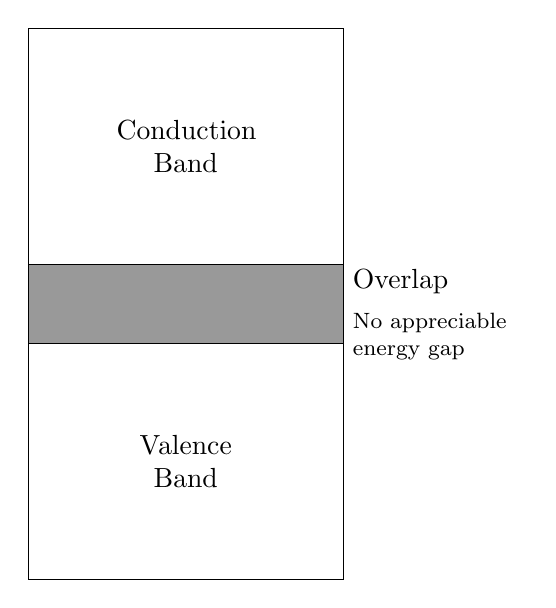
\begin{tikzpicture}
        %% conduction band
        \draw (-2,0.5) rectangle (2,3.5);
        \node[anchor=center,text centered,text width=5em] at (0,2) {Conduction Band};
        %% overlap
        \draw[fill=white!60!black] (-2,-0.5) rectangle (2,+0.5);
        \node[anchor=south west] at (2,0) {Overlap};
        \node[anchor=north west,text width=6em,font=\footnotesize] at (2,0) {No appreciable energy gap};
        %% Valence band
        \draw (-2,-0.5) rectangle (2,-3.5);
        \node[anchor=center,text centered,text width=4em] at (0,-2) {Valence Band};
    \end{tikzpicture}
    \end{center}
    The substance is best classified as:
    \begin{multicols}{2}
    \begin{choices}
        \wrongchoice{an insulator}
        \wrongchoice{a semiconductor}
      \correctchoice{a conductor}
        \wrongchoice{a nonmetal}
    \end{choices}
    \end{multicols}
\end{question}
}

\element{nysed}{
\begin{question}{June2001-Q98}
    Magnetic-card door locks utilize many electronic components on one small piece of semiconductor material.
    This combination of components on a single chip is called:
    \begin{choices}
        \wrongchoice{a transistor}
      \correctchoice{an integrated circuit}
        \wrongchoice{a printed circuit board}
        \wrongchoice{a diode}
    \end{choices}
\end{question}
}

\element{nysed}{
\begin{question}{June2001-Q99}
    The Band Model has replaced the Electron-sea Model of conduction because the Electron-sea Model:
    \begin{choices}
        \wrongchoice{only works for gases}
        \wrongchoice{only works for liquids}
        \wrongchoice{does not account for the conduction properties of metals}
      \correctchoice{does not account for the conduction properties of semiconductors}
    \end{choices}
\end{question}
}

%% boxes with anchor to previous
\element{nysed}{
\begin{question}{June2001-Q100}
    The diagram below shows a portion of the Periodic Table of the Elements.
    \begin{center}
        %% NOTE: tikz with nodes and anchor to each other
        %% NOTE: check cpo for example
        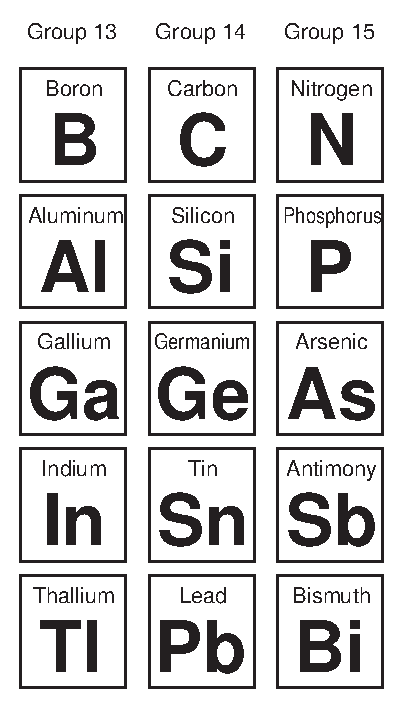
\includegraphics[keepaspectratio,scale=0.85]{June2001-Q100}
    \end{center}
    Based on the information in this diagram,
        which three elements could all be used as doping agents to produce the holes of a $P$-type semiconductor?
    \begin{choices}
      \correctchoice{boron, aluminum, and gallium}
        \wrongchoice{boron, carbon, and nitrogen}
        \wrongchoice{thallium, germanium, and phosphorus}
        \wrongchoice{nitrogen, phosphorus, and arsenic}
    \end{choices}
\end{question}
}

\element{nysed}{
\begin{question}{June2001-Q101}
    The diagram below shows a circuit with a battery applying a potential difference across a $P$-type semiconductor.
    \begin{center}
    \ctikzset{bipoles/length=1.00cm}
    \begin{circuitikz}
        \draw (6,0) to [battery] (0,0) to (0,2) to  (6,2) to (6,0);
        \node[draw,fill=white,anchor=center,text centered,text width=6em] at (3,2) {P-type semiconductor};
        \node[anchor=south west] at (0,2) {Left};
        \node[anchor=south east] at (6,2) {Right};
        \node[anchor=south west] at (3.2,0) {$-$};
        \node[anchor=south east] at (2.8,0) {$+$};
    \end{circuitikz}
    \end{center}
    The majority charge carriers in the semiconductor are:
    \begin{choices}
        \wrongchoice{negative electrons moving to the right}
        \wrongchoice{negative electrons moving to the left}
      \correctchoice{positive holes moving to the right}
        \wrongchoice{positive holes moving to the left}
    \end{choices}
\end{question}
}

\element{nysed}{
\begin{question}{June2001-Q102}
    Which diagram best represents a diode?
    \begin{multicols}{2}
    \begin{choices}
        \AMCboxDimensions{down=-0.8cm}
        \ctikzset{bipoles/length=0.75cm}
        \wrongchoice{
            \begin{circuitikz}
                \draw[dashed,white!60!black] (-1,-1.5) rectangle (1,0.5);
                \node[pnp,rotate=90] (pnp) at (0,0) {};
            \end{circuitikz}
        }
        \wrongchoice{
            \begin{circuitikz}
                \draw[dashed,white!60!black] (-1,-1.5) rectangle (1,0.5);
                \node[npn,rotate=270,xscale=-1] (npn) at (0,0) {};
            \end{circuitikz}
        }
        \wrongchoice{
            \begin{circuitikz}
                \draw[dashed,white!60!black] (-1,-1) rectangle (1,1);
                \draw (-1,0) -- (1,0);
                \draw (-0.5,0) to [full diode] (0,0);
                \draw (+0.5,0) to [full diode] (0,0);
            \end{circuitikz}
        }
        \correctchoice{
            \begin{circuitikz}
                \draw[dashed,white!60!black] (-1,-1) rectangle (1,1);
                \draw (-1,0) to [full diode] (1,0);
            \end{circuitikz}
        }
    \end{choices}
    \end{multicols}
\end{question}
}

\element{nysed}{
\begin{question}{June2001-Q103}
    In the $P$-$N$ junction region of an operating diode,
        an electric field barrier is produced by free electrons in the:
    \begin{choices}
      \correctchoice{$N$-type material crossing into the $P$-type material}
        \wrongchoice{$N$-type material going away from the $P$-type material}
        \wrongchoice{$P$-type material crossing into the $N$-type material}
        \wrongchoice{$P$-type material going away from the $N$-type material}
    \end{choices}
\end{question}
}

\element{nysed}{
\begin{question}{June2001-Q104}
    In a $P$-$N$-$P$ transistor,
        what is the function of the two types of material?
    \begin{choices}
         \wrongchoice{The $N$-type material functions as the base, and the $P$-type material is both emitter and collector.}
         \wrongchoice{The $N$-type material functions as both base and emitter, and the $P$-type material is the collector.}
       \correctchoice{The $N$-type material functions as the emitter, and the $P$-type material is both base and collector.}
         \wrongchoice{The $N$-type material functions as the collector, and the $P$-type material is both emitter and base.}
    \end{choices}
\end{question}
}

\element{nysed}{
\begin{question}{June2001-Q105}
    As the temperature of a semiconductor increases,
        the number of holes in the valence band will:
    \begin{choices}
      \correctchoice{decrease}
        \wrongchoice{increase}
        \wrongchoice{remain the same}
    \end{choices}
\end{question}
}


%% Section Jan2001
%%--------------------
\newcommand{\nysedJanTwentyZeroOneQNinetySix}{
\ctikzset{bipoles/length=0.80cm}
\begin{circuitikz}
    \draw (0,0) to [thick,full diode] (4,0);
    \node[anchor=south] at (1,0) {$X$};
    \node[anchor=south] at (3,0) {$Z$};
\end{circuitikz}
}

\element{nysed}{
\begin{question}{Jan2001-Q96}
    Below is a diagram of a semiconductor.
    \begin{center}
        \nysedJanTwentyZeroOneQNinetySix
    \end{center}
    The semiconductor represented in the diagram is a:
    \begin{multicols}{2}
    \begin{choices}
        \wrongchoice{transistor}
        \wrongchoice{resistor}
        \wrongchoice{emitter}
      \correctchoice{diode}
    \end{choices}
    \end{multicols}
\end{question}
}

\element{nysed}{
\begin{question}{Jan2001-Q97}
    Below is a diagram of a semiconductor.
    \begin{center}
        \nysedJanTwentyZeroOneQNinetySix
    \end{center}
    This device is called a semiconductor because:
    \begin{choices}
      \correctchoice{positive holes move from $X$ to $Z$}
        \wrongchoice{positive holes move from $Z$ to $X$}
        \wrongchoice{negative holes flow from $Z$ to $X$}
        \wrongchoice{negative electrons flow from $X$ to $Z$}
    \end{choices}
\end{question}
}

\element{nysed}{
\begin{question}{Jan2001-Q98}
    Below is a diagram of a semiconductor.
    \begin{center}
        \nysedJanTwentyZeroOneQNinetySix
    \end{center}
    The part of the semiconductor labeled $X$ is called the:
    \begin{multicols}{2}
    \begin{choices}
        \wrongchoice{cathode}
        \wrongchoice{emitter}
      \correctchoice{anode}
        \wrongchoice{collector}
    \end{choices}
    \end{multicols}
\end{question}
}

\element{nysed}{
\begin{question}{Jan2001-Q99}
    A diode can be used in a circuit to:
    \begin{choices}
        \wrongchoice{convert direct current to alternating current}
      \correctchoice{convert alternating current to direct current}
        \wrongchoice{amplify voltage}
        \wrongchoice{amplify current}
    \end{choices}
\end{question}
}

\element{nysed}{
\begin{question}{Jan2001-Q100}
    Which diagram represents an $N$--$P$--$N$ transistor?
    \begin{multicols}{2}
    \begin{choices}[o]
        \AMCboxDimensions{down=-0.75cm}
        \wrongchoice{
            \begin{circuitikz}
                \draw[dashed,white!60!black] (-1,-1.5) rectangle (1,0.5);
                \node[pnp,rotate=270,xscale=-1] (pnp) at (0,0) {};
            \end{circuitikz}
        }
        \correctchoice{
            \begin{circuitikz}
                \draw[dashed,white!60!black] (-1,-1.5) rectangle (1,0.5);
                \node[npn,rotate=270,xscale=-1] (npn) at (0,0) {};
            \end{circuitikz}
        }
        \wrongchoice{
            \begin{circuitikz}[american voltages]
                \draw[dashed,white!60!black] (-1,-1.5) rectangle (1,0.5);
                \draw (0,-1.5) to [battery1,v=$ $] (0,0.5);
                %% arrows??
                \draw[<-,thick] (0,-0.5) ++ (5:1.2em) -- ++(45:1.5em);
                \draw[<-,thick] (0,-0.5) ++(55:1.2em) -- ++(45:1.5em);
            \end{circuitikz}
        }
        \wrongchoice{
            \begin{circuitikz}[american voltages]
                \draw[dashed,white!60!black] (-1,-1.5) rectangle (1,0.5);
                \draw (0,0.5) to [R,v=$ $] (0,-1.5);
                %% arrows??
                \draw[<-,thick] (0,-0.5) ++ (5:1.2em) -- ++(45:1.5em);
                \draw[<-,thick] (0,-0.5) ++(55:1.2em) -- ++(45:1.5em);
            \end{circuitikz}
        }
    \end{choices}
    \end{multicols}
\end{question}
}

\element{nysed}{
\begin{question}{Jan2001-Q101}
    An impurity that is added to a semiconductor in order to provide holes is classified as:
    \begin{multicols}{2}
    \begin{choices}
        \wrongchoice{a donor}
        \wrongchoice{a receptor}
      \correctchoice{an acceptor}
        \wrongchoice{a bias}
    \end{choices}
    \end{multicols}
\end{question}
}

\element{nysed}{
\begin{question}{Jan2001-Q102}
    Current in a semiconductor is caused by the movement of:
    \begin{choices}
        \wrongchoice{electrons, only}
        \wrongchoice{holes, only}
        \wrongchoice{isotopes}
      \correctchoice{both electrons and holes}
    \end{choices}
\end{question}
}

\element{nysed}{
\begin{question}{Jan2001-Q103}
    In a $P$--$N$--$P$ transistor,
        the section that has the thinnest segment is the:
    \begin{multicols}{2}
    \begin{choices}
        \wrongchoice{emitter}
        \wrongchoice{acceptor}
        \wrongchoice{collector}
      \correctchoice{base}
    \end{choices}
    \end{multicols}
\end{question}
}

\element{nysed}{
\begin{question}{Jan2001-Q104}
    Compared to the current flow when a forward bias is applied to a $P$--$N$ junction,
        the current flow when a reverse bias is applied to a $P$--$N$ junction is:
    \begin{multicols}{2}
    \begin{choices}
      \correctchoice{less}
        \wrongchoice{greater}
        \wrongchoice{the same}
    \end{choices}
    \end{multicols}
\end{question}
}

\element{nysed}{
\begin{question}{Jan2001-Q105}
    Donor materials are added to semiconductors so that the number of available electrons will:
    \begin{multicols}{2}
    \begin{choices}
        \wrongchoice{decrease}
      \correctchoice{increase}
        \wrongchoice{remain the same}
    \end{choices}
    \end{multicols}
\end{question}
}


%% Section June2000
%%--------------------
\element{nysed}{
\begin{question}{June2000-Q96}
    Which statement best explains how the resistivity of glass compares to the resistivity of copper?
    \begin{choices}
        \wrongchoice{Glass has a lower resistivity and is a poor conductor.}
        \wrongchoice{Glass has a lower resistivity and is a good conductor.}
      \correctchoice{Glass has a higher resistivity and is a poor conductor.}
        \wrongchoice{Glass has a higher resistivity and is a good conductor.}
    \end{choices}
\end{question}
}

\element{nysed}{
\begin{question}{June2000-Q97}
    Metals that are excellent conductors have valence electrons that are:
    \begin{choices}
        \wrongchoice{difficult to dislodge and difficult to move through the crystal}
        \wrongchoice{difficult to dislodge but easy to move through the crystal}
        \wrongchoice{easy to dislodge but difficult to move through the crystal}
      \correctchoice{easy to dislodge and easy to move through the crystal}
    \end{choices}
\end{question}
}

\element{nysed}{
\begin{question}{June2000-Q98}
    Which energy band diagram best represents a semiconductor?
    \begin{multicols}{2}
    \begin{choices}
        \AMCboxDimensions{down=-0.5cm}
        \wrongchoice{
            \begin{tikzpicture}
                %% NOTE: TODO: draw tikz
            \end{tikzpicture}
        }
        \wrongchoice{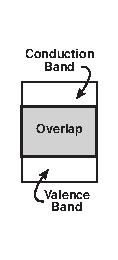
\includegraphics[keepaspectratio,scale=0.85]{June2000-Q98-A}}
        \wrongchoice{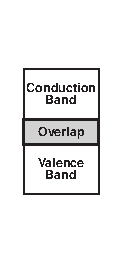
\includegraphics[keepaspectratio,scale=0.85]{June2000-Q98-B}}
      \correctchoice{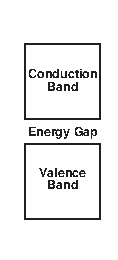
\includegraphics[keepaspectratio,scale=0.85]{June2000-Q98-C}}
        \wrongchoice{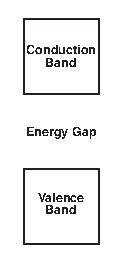
\includegraphics[keepaspectratio,scale=0.85]{June2000-Q98-D}}
    \end{choices}
    \end{multicols}
\end{question}
}

\element{nysed}{
\begin{question}{June2000-Q99}
    Alternating current from a wall outlet can be converted to direct current by:
    \begin{choices}
        \wrongchoice{an $N$-type semiconductor}
        \wrongchoice{a $P$-type semiconductor}
        \wrongchoice{an emitter}
      \correctchoice{a diode}
    \end{choices}
\end{question}
}

\element{nysed}{
\begin{question}{June2000-Q100}
    The table below lists the number of valence electrons for some elements.
    \begin{center}
    \begin{tabu}{X[r]X[c]}
        \toprule
                    & Number of \\
        Element     & of Valence Electrons \\
        \midrule
        antimony    & 5 \\
        silicon     & 4 \\
        germanium   & 4 \\
        aluminum    & 3 \\
        \bottomrule
    \end{tabu}
    \end{center}
    Which combination of elements could be used to make an $N$-type semiconductor?
    \begin{choices}
      \correctchoice{antimony and silicon}
        \wrongchoice{silicon and germanium}
        \wrongchoice{germanium and aluminum}
        \wrongchoice{aluminum and antimony}
    \end{choices}
\end{question}
}

\element{nysed}{
\begin{question}{June2000-Q101}
    Which diagram below shows a correctly labeled $P$-$N$-$P$ transistor?
    \begin{choices}[o]
        \AMCboxDimensions{down=-0.5cm}
        \correctchoice{
            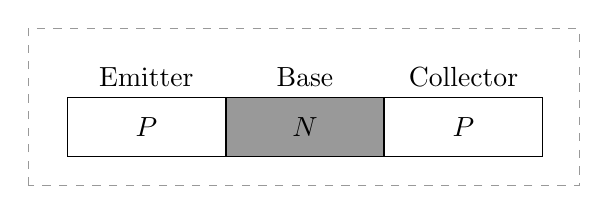
\begin{tikzpicture}
                \draw[dashed,white!60!black] (-1.5,-0.75) rectangle (5.5,1.25);
                %% Emitter/Base/Collector
                \node[anchor=center,draw,minimum width=2cm,minimum height=0.75cm] (L) at (0,0) {$P$};
                \node[anchor=west,draw,fill=white!60!black,minimum width=2cm,minimum height=0.75cm] (M) at (L.east) {$N$};
                \node[anchor=west,draw,minimum width=2cm,minimum height=0.75cm] (R) at (M.east) {$P$};
                %% labels
                \node[anchor=south] at (L.north) {Emitter};
                \node[anchor=south] at (M.north) {Base};
                \node[anchor=south] at (R.north) {Collector};
            \end{tikzpicture}
        }
        \wrongchoice{
            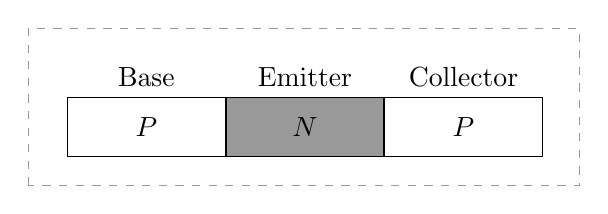
\begin{tikzpicture}
                \draw[dashed,white!60!black] (-1.5,-0.75) rectangle (5.5,1.25);
                %% Emitter/Base/Collector
                \node[anchor=center,draw,minimum width=2cm,minimum height=0.75cm] (L) at (0,0) {$P$};
                \node[anchor=west,draw,fill=white!60!black,minimum width=2cm,minimum height=0.75cm] (M) at (L.east) {$N$};
                \node[anchor=west,draw,minimum width=2cm,minimum height=0.75cm] (R) at (M.east) {$P$};
                %% labels
                \node[anchor=south] at (L.north) {Base};
                \node[anchor=south] at (M.north) {Emitter};
                \node[anchor=south] at (R.north) {Collector};
            \end{tikzpicture}
        }
        \wrongchoice{
            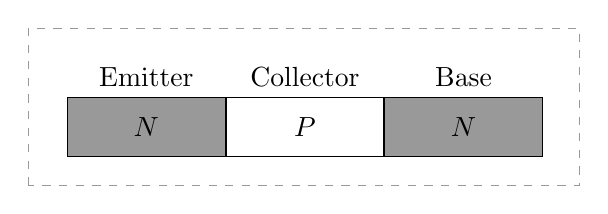
\begin{tikzpicture}
                \draw[dashed,white!60!black] (-1.5,-0.75) rectangle (5.5,1.25);
                %% Emitter/Base/Collector
                \node[anchor=center,draw,fill=white!60!black,minimum width=2cm,minimum height=0.75cm] (L) at (0,0) {$N$};
                \node[anchor=west,draw,minimum width=2cm,minimum height=0.75cm] (M) at (L.east) {$P$};
                \node[anchor=west,draw,fill=white!60!black,minimum width=2cm,minimum height=0.75cm] (R) at (M.east) {$N$};
                %% labels
                \node[anchor=south] at (L.north) {Emitter};
                \node[anchor=south] at (M.north) {Collector};
                \node[anchor=south] at (R.north) {Base};
            \end{tikzpicture}
        }
        \wrongchoice{
            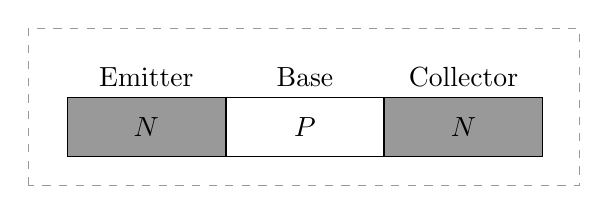
\begin{tikzpicture}
                \draw[dashed,white!60!black] (-1.5,-0.75) rectangle (5.5,1.25);
                %% Emitter/Base/Collector
                \node[anchor=center,draw,fill=white!60!black,minimum width=2cm,minimum height=0.75cm] (L) at (0,0) {$N$};
                \node[anchor=west,draw,minimum width=2cm,minimum height=0.75cm] (M) at (L.east) {$P$};
                \node[anchor=west,draw,fill=white!60!black,minimum width=2cm,minimum height=0.75cm] (R) at (M.east) {$N$};
                %% labels
                \node[anchor=south] at (L.north) {Emitter};
                \node[anchor=south] at (M.north) {Base};
                \node[anchor=south] at (R.north) {Collector};
            \end{tikzpicture}
        }
    \end{choices}
\end{question}
}

\element{nysed}{
\begin{question}{June2000-Q102}
    The diagram below represents an $N$-type semiconductor connected to a battery.
    Which phrase best describes the majority charge carriers within the semiconductor?
    \begin{choices}
        \wrongchoice{electrons moving to the left}
      \correctchoice{electrons moving to the right}
        \wrongchoice{holes moving to the left}
        \wrongchoice{holes moving to the right}
    \end{choices}
\end{question}
}

\element{nysed}{
\begin{question}{June2000-Q103}
    In the circuit diagram below,
        a diode and an incandescent light bulb are connected in series with a source of alternating current having a frequency of \SI{60}{\hertz}.
    The diagram below represents an $N$-type semiconductor connected to a battery.
    Which phrase best describes the majority charge carriers within the semiconductor?
    \begin{center}
    \ctikzset{bipoles/length=1.00cm}
    \begin{circuitikz}
        \draw (0,0) to [sV,l={a.c. source}] (0,3) to [full diode,l={Diode}] (3,3) to [R,l={light bulb}] (3,0) to (0,0);
    \end{circuitikz}
    \end{center}
    How many times per second does a maximum current exist in the light bulb?
    \begin{multicols}{4}
    \begin{choices}
        \wrongchoice{\num{30}}
      \correctchoice{\num{60}}
        \wrongchoice{\num{120}}
        \wrongchoice{\num{240}}
    \end{choices}
    \end{multicols}
\end{question}
}

\element{nysed}{
\begin{question}{June2000-Q104}
    Which part of an $N-P-N$ transistor is forward biased?
    \begin{choices}
        \wrongchoice{an integrated circuit}
        \wrongchoice{a parallel circuit}
      \correctchoice{an emitter-base combination}
        \wrongchoice{a collector-base combination}
    \end{choices}
\end{question}
}

\element{nysed}{
\begin{question}{June2000-Q105}
    The transistor shown in the circuit diagram below is being used as an amplifier.
    \begin{center}
    \ctikzset{bipoles/length=1.00cm}
    \begin{circuitikz}
        \draw (0,3) node[npn,rotate=270,xscale=-1] (npn) {}
            (npn.base) to [short,i=$I_b$] (0,0) to (-2,0) to (-2,3) to [short,i=$I_e$] (npn.emitter);
        \draw (-2,2) to [battery1] (-2,0); 
        \draw (2,0) to [battery] (2,2); 
        \draw (npn.collector) to [short,i=$I_c$] (2,3) to (2,0) to (0,0);
    \end{circuitikz}
    \end{center}
    When the emitter current ($I_e$) increases, the collector current ($I_c$):
    \begin{choices}
        \wrongchoice{decreases}
      \correctchoice{increases}
        \wrongchoice{remains the same}
    \end{choices}
\end{question}
}


%% Section June1999
%%--------------------
\element{nysed}{
\begin{question}{June1999-Q96}
    Which symbol correctly represents a transistor?
    \begin{multicols}{2}
    \begin{choices}
        %% NOTE: I changed these options, circuitikz has no way to write incorrect symbols
        \AMCboxDimensions{down=-0.8cm}\small
        \ctikzset{bipoles/length=0.75cm}
        \wrongchoice{
            \begin{circuitikz}
                \draw[dashed,white!60!black] (-1.6,-1) rectangle (1.6,1);
                \draw (-1.5,0) to [thick,full diode] (1.5,0);
                \node[anchor=south west] at (-1.5,0) {Anode};
                \node[anchor=south east,xshift=1ex] at (+1.5,0) {Cathode};
            \end{circuitikz}
        }
        \wrongchoice{
            \begin{circuitikz}
                \draw[dashed,white!60!black] (-1.6,-1) rectangle (1.6,1);
                \draw (+1.5,0) to [thick,full diode] (-1.5,0);
                \node[anchor=south west] at (-1.5,0) {Anode};
                \node[anchor=south east,xshift=1ex] at (+1.5,0) {Cathode};
            \end{circuitikz}
        }
        \correctchoice{
            \begin{circuitikz}
                \draw[dashed,white!60!black] (-1.6,-1) rectangle (1.6,1);
                \node[pnp,rotate=90] (pnp) at (0,0) {};
                \draw (pnp.C) to (+1.5,0) node[anchor=south east] {Collector};
                \draw (pnp.E) to (-1.5,0) node[anchor=south west] {Emitter};
            \end{circuitikz}
        }
        \wrongchoice{
            \begin{circuitikz}
                \draw[dashed,white!60!black] (-1.6,-1) rectangle (1.6,1);
                \node[npn,rotate=270,xscale=-1] (npn) at (0,0) {};
                \draw (npn.E) to (-1.5,0) node[anchor=south west] {Collector};
                \draw (npn.C) to (+1.5,0) node[anchor=south east] {Emitter};
            \end{circuitikz}
        }
    \end{choices}
    \end{multicols}
\end{question}
}

\element{nysed}{
\begin{question}{June1999-Q97}
    For a solid to be an efficient carrier of electric current,
        its electronic conduction band should:
    \begin{choices}
      \correctchoice{overlap its valence band}
        \wrongchoice{have a large gap with its valence band}
        \wrongchoice{be smaller than its valence band}
        \wrongchoice{be at a higher energy level than its valence band}
    \end{choices}
\end{question}
}

\newcommand{\nysedJuneNineteenNinetyNineQNinetyEight}{
\ctikzset{bipoles/length=1.00cm}
\begin{circuitikz}
    %% circuit
    \draw (0,0) to [battery] (6,0) to (6,3) to  (0,3) to (0,0);
    %% NP diode
    \node[draw,thick,fill=white,minimum width=2cm,minimum height=1.5cm,anchor=east] (A) at (3,3) {};
    \node[draw,thick,fill=white,minimum width=2cm,minimum height=1.5cm,anchor=west] (C) at (3,3) {};
    %% labels
    \node[anchor=south east] at (2.8,0) {$-$};
    \node[anchor=south west] at (3.2,0) {$+$};
    \node[anchor=north east] at (2.8,0) {$D$};
    \node[anchor=north west] at (3.2,0) {$E$};
    \node[anchor=south] at (A.north) {$A$};
    \node[anchor=south] at (C.north) {$B$};
    \fill (0,0) circle (2pt) node[anchor=north] {$C$};
    \fill (6,0) circle (2pt) node[anchor=north] {$F$};
    %% negative
    \node[anchor=north west] at (A.north west) {electrons};
    \foreach \y in {24,27,30,33,36}
        \draw[thick] (2.75,\y mm) -- ++(0:4pt);
    \foreach \y in {1,2,3,4}
        \draw[thick] ({2+0.5*rand},{3+0.5*rand}) -- ++(0:4pt);
    %% holes
    \node[anchor=north east] at (C.north east) {holes};
    \foreach \y in {24,27,30,33,36}
        \draw (3.25,\y mm) circle (2pt);
    \foreach \y in {1,2,3,4}
        \draw[thick] ({4+0.5*rand},{3+0.5*rand}) circle (2pt);
\end{circuitikz}
}

\element{nysed}{
\begin{question}{June1999-Q98}
    The diagram below represents a germanium semiconductor device.
    \begin{center}
        \nysedJuneNineteenNinetyNineQNinetyEight
    \end{center}
    In the diagram, section $A$ represents the:
    \begin{choices}
      \correctchoice{$N$-type germanium}
        \wrongchoice{$P$-type germanium}
        \wrongchoice{anode}
        \wrongchoice{diode}
    \end{choices}
\end{question}
}

\element{nysed}{
\begin{question}{June1999-Q99}
    The diagram below represents a germanium semiconductor device.
    \begin{center}
        \nysedJuneNineteenNinetyNineQNinetyEight
    \end{center}
    The bias of the $P$-$N$ junction shown in the diagram is:
    \begin{multicols}{2}
    \begin{choices}
        \wrongchoice{$C$ to $D$}
        \wrongchoice{$E$ to $F$}
        \wrongchoice{reverse}
      \correctchoice{foreward}
    \end{choices}
    \end{multicols}
\end{question}
}

\element{nysed}{
\begin{question}{June1999-Q100}
    The diagram below shows an $N$-type semiconductor connected to a battery and a switch.
    \begin{center}
    \ctikzset{bipoles/length=1.00cm}
    \begin{circuitikz}
        \draw (0,0) to [cspst,l={switch}] (3,0) to [battery] (6,0) to (6,2) to  (0,2) to (0,0);
        \node[draw,fill=white,anchor=center,text centered,text width=6em] (N) at (3,2) {$N$-type semiconductor};
        \node[anchor=south east] at (4.3,0) {$-$};
        \node[anchor=south west] at (4.8,0) {$+$};
    \end{circuitikz}
    \end{center}
    When the switch is closed, conduction in the semiconductor consists of:
    \begin{choices}
      \correctchoice{majority charge carriers moving toward the right and minority charge carriers moving toward the left.}
        \wrongchoice{majority charge carriers moving toward the left and minority charge carriers moving toward the right.}
        \wrongchoice{both majority and minority charge carriers moving toward the right.}
        \wrongchoice{both majority and minority charge carriers moving toward the left.}
    \end{choices}
\end{question}
}

\element{nysed}{
\begin{question}{June1999-Q101}
    The circuit in the diagram below contains three \SI{6}{\ohm} resistors,
        four diodes, a \SI{12}{\volt} batter, and an ammeter.
    \begin{center}
    \ctikzset{bipoles/length=1.00cm}
    \begin{circuitikz}
        \draw (0,0) to [battery,l=\SI{12}{\volt}] (0,4) to [ammeter] (2,4) to [R,l=\SI{6.0}{\ohm}] (2,2) to (2,1) to [full diode] (2,0) to (0,0);
        \draw (2,4) to (4,4) to [R,l=\SI{6}{\ohm}] (4,2) to (4,0) to (2,0);
        \draw (4,4) to (6,4) to [R,l=\SI{6}{\ohm}] (6,2) to (6,1) to [full diode] (6,0) to (4,0);
        \draw (4,0) to (4,1) to [full diode] (4,2);
        \draw (2,0) to (2,1) to [full diode] (2,2);
    \end{circuitikz}
    \end{center}
    The current measured by the ammeter is:
    \begin{multicols}{2}
    \begin{choices}
        \wrongchoice{\SI{0.7}{\ampere}}
      \correctchoice{\SI{2}{\ampere}}
        \wrongchoice{\SI{6}{\ampere}}
        \wrongchoice{\SI{4}{\ampere}}
    \end{choices}
    \end{multicols}
\end{question}
}

\element{nysed}{
\begin{question}{June1999-Q102}
    In an $N$-$P$-$N$ transistor,
        approximately what percentage of the electrons pass from the emitter through the base and to the collector?
    \begin{multicols}{2}
    \begin{choices}
        \wrongchoice{\SI{15}{\percent}}
        \wrongchoice{\SI{2}{\percent}}
        \wrongchoice{\SI{50}{\percent}}
      \correctchoice{\SI{98}{\percent}}
    \end{choices}
    \end{multicols}
\end{question}
}

\element{nysed}{
\begin{question}{June1999-Q103}
    Doping a semiconducting material with a donor impurity results in:
    \begin{choices}
        \wrongchoice{an excess of positive holes}
        \wrongchoice{a deficiency of free electrons}
      \correctchoice{an excess of free electrons}
        \wrongchoice{a deficiency of atoms}
    \end{choices}
\end{question}
}

\element{nysed}{
\begin{question}{June1999-Q104}
    As the temperature of a solid semiconductor increases,
        its conductivity:
    \begin{choices}
        \wrongchoice{decreases}
      \correctchoice{increases}
        \wrongchoice{remains the same}
    \end{choices}
\end{question}
}

\element{nysed}{
\begin{question}{June1999-Q105}
    When a semiconductor in a circuit at room temperature is replaced by an insulator,
        the resistance of that section of the circuit:
    \begin{choices}
        \wrongchoice{decreases}
      \correctchoice{increases}
        \wrongchoice{remains the same}
    \end{choices}
\end{question}
}


%% Section June1998
%%--------------------
\element{nysed}{
\begin{question}{June1998-Q96}
    The diagram below represents the wave form and phase of an alternating current signal.
    \begin{center}
    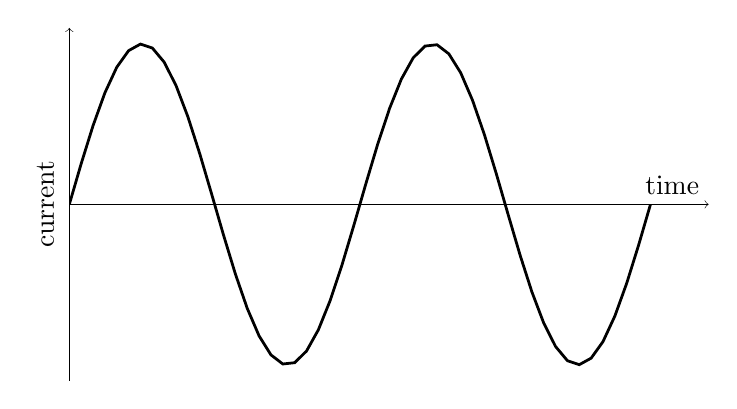
\begin{tikzpicture}
        \begin{axis}[
            axis y line=left,
            axis x line=middle,
            axis line style={->},
            xlabel={time},
            xtick=\empty,
            ylabel={current},
            ytick=\empty,
            xmin=0,xmax=11,
            ymin=-1.1,ymax=1.1,
            width=0.8\columnwidth,
            height=0.5\columnwidth,
            very thin,
        ]
        \addplot[line width=1pt,domain=0:10,samples=50]{sin(72*x)};
        \end{axis}
    \end{tikzpicture}
    \end{center}
    Which graph best represents the wave form and phase of this signal after it has passed through a diode rectifier?
    \begin{multicols}{2}
    \begin{choices}
        \AMCboxDimensions{down=-2.5em}
        \wrongchoice{
            \begin{tikzpicture}
                \begin{axis}[
                    axis y line=left,
                    axis x line=middle,
                    axis line style={->},
                    xlabel={time},
                    xtick=\empty,
                    ylabel={current},
                    ytick=\empty,
                    xmin=0,xmax=11,
                    ymin=-1.1,ymax=1.1,
                    width=\columnwidth,
                    very thin,
                ]
                \addplot[line width=1pt,domain=0:10,samples=50]{sin(72*x)};
                \end{axis}
            \end{tikzpicture}
        }
        \wrongchoice{
            \begin{tikzpicture}
                \begin{axis}[
                    axis y line=left,
                    axis x line=middle,
                    axis line style={->},
                    xlabel={time},
                    xtick=\empty,
                    x label style={anchor=north east},
                    ylabel={current},
                    ytick=\empty,
                    xmin=0,xmax=11,
                    ymin=-1.1,ymax=1.1,
                    width=\columnwidth,
                    very thin,
                ]
                \addplot[line width=1pt,domain=0:10,samples=50]{-1*sin(72*x)};
                \end{axis}
            \end{tikzpicture}
        }
        \correctchoice{
            \begin{tikzpicture}
                \begin{axis}[
                    axis y line=left,
                    axis x line=middle,
                    axis line style={->},
                    xlabel={time},
                    xtick=\empty,
                    x label style={anchor=north east},
                    ylabel={current},
                    ytick=\empty,
                    xmin=0,xmax=11,
                    ymin=-1.1,ymax=1.1,
                    width=\columnwidth,
                    very thin,
                ]
                \clip (axis cs:0,0) rectangle (axis cs:10,1);
                \addplot[line width=1pt,domain=0:10,samples=50]{sin(72*x)};
                \end{axis}
            \end{tikzpicture}
        }
        \wrongchoice{
            \begin{tikzpicture}
                \begin{axis}[
                    axis y line=left,
                    axis x line=middle,
                    axis line style={->},
                    xlabel={time},
                    xtick=\empty,
                    ylabel={current},
                    ytick=\empty,
                    xmin=0,xmax=11,
                    ymin=-1.1,ymax=1.1,
                    width=\columnwidth,
                    very thin,
                ]
                \clip (axis cs:0,0) rectangle (axis cs:10,-1);
                \addplot[line width=1pt,domain=0:10,samples=50]{-1*sin(72*x)};
                \end{axis}
            \end{tikzpicture}
        }
    \end{choices}
    \end{multicols}
\end{question}
}

\element{nysed}{
\begin{question}{June1998-Q97}
    Which graph best represents the relationship between current and potential difference for a forward-biased diode?
    \begin{multicols}{2}
    \begin{choices}
        \AMCboxDimensions{down=-3.5em}
        %% ANS is A
        \correctchoice{
            \begin{tikzpicture}
                \begin{axis}[
                    axis y line=left,
                    axis x line=bottom,
                    axis line style={->},
                    xlabel={potential},
                    x unit=\si{\volt},
                    xtick={8},
                    xticklabels={-0.7},
                    ylabel={current},
                    y unit=\si{\milli\ampere},
                    ytick=\empty,
                    xmin=0,xmax=11,
                    ymin=0,ymax=11,
                    width=\columnwidth,
                    very thin,
                ]
                \draw[line width=1pt] (axis cs:0,0) to[out=0,in=270,tension=10] (axis cs:7.9,10);
                \draw[dashed] (axis cs:8,0) -- (axis cs:8,10);
                \end{axis}
            \end{tikzpicture}
        }
        \wrongchoice{
            \begin{tikzpicture}
                \begin{axis}[
                    axis y line=left,
                    axis x line=bottom,
                    axis line style={->},
                    xlabel={potential},
                    x unit=\si{\volt},
                    xtick={8},
                    xticklabels={-0.7},
                    ylabel={current},
                    y unit=\si{\milli\ampere},
                    ytick=\empty,
                    xmin=0,xmax=11,
                    ymin=0,ymax=11,
                    width=\columnwidth,
                    very thin,
                ]
                \draw[line width=1pt] (axis cs:0,10) to[out=0,in=90,tension=3] (axis cs:7.9,0);
                \draw[dashed] (axis cs:8,0) -- (axis cs:8,10);
                \end{axis}
            \end{tikzpicture}
        }
        \wrongchoice{
            \begin{tikzpicture}
                \begin{axis}[
                    axis y line=left,
                    axis x line=bottom,
                    axis line style={->},
                    xlabel={potential},
                    x unit=\si{\volt},
                    xtick={8},
                    xticklabels={-0.7},
                    ylabel={current},
                    y unit=\si{\milli\ampere},
                    ytick=\empty,
                    xmin=0,xmax=11,
                    ymin=0,ymax=11,
                    width=\columnwidth,
                    very thin,
                ]
                \draw[line width=1pt] (axis cs:8,0) to[out=180,in=270,tension=10] (axis cs:0.15,10);
                \draw[dashed] (axis cs:8,0) -- (axis cs:8,10);
                \end{axis}
            \end{tikzpicture}
        }
        \wrongchoice{
            \begin{tikzpicture}
                \begin{axis}[
                    axis y line=left,
                    axis x line=bottom,
                    axis line style={->},
                    xlabel={potential},
                    x unit=\si{\volt},
                    xtick={8},
                    xticklabels={-0.7},
                    ylabel={current},
                    y unit=\si{\milli\ampere},
                    ytick=\empty,
                    xmin=0,xmax=11,
                    ymin=0,ymax=11,
                    width=\columnwidth,
                    very thin,
                ]
                \addplot[line width=1pt,mark=\empty] plot coordinates { (0,10) (8,8) (10,0) };
                \draw[dashed] (axis cs:8,0) -- (axis cs:8,10);
                \end{axis}
            \end{tikzpicture}
        }
    \end{choices}
    \end{multicols}
\end{question}
}

\element{nysed}{
\begin{question}{June1998-Q98}
    A circuit is shown in the diagram below.
    \begin{center}
    \ctikzset{bipoles/length=1.00cm}
    \begin{circuitikz}
        %\draw (0,0) to [battery1,v=$ $] (3,0);
        \draw (0,0) to [battery1] (3,0);
        \node[anchor=south east] at (1.4,0) {$-$};
        \node[anchor=south west] at (1.6,0) {$+$};
        \draw (0,0) to (0,2) to [thick,full diode] (3,2) to (3,0);
    \end{circuitikz}
    \end{center}
    The current in the electronic device is classified as:
    \begin{multicols}{2}
    \begin{choices}
      \correctchoice{reverse biased}
        \wrongchoice{forward biased}
        \wrongchoice{unbiased}
        \wrongchoice{transistorized}
    \end{choices}
    \end{multicols}
\end{question}
}

\element{nysed}{
\begin{question}{June1998-Q99}
    Compared to the number of holes in an $N$-type semiconductor,
        the number of free electrons is:
    \begin{multicols}{3}
    \begin{choices}
        \wrongchoice{less}
      \correctchoice{greater}
        \wrongchoice{the same}
    \end{choices}
    \end{multicols}
\end{question}
}

\element{nysed}{
\begin{question}{June1998-Q100}
    The primary source of holes in $P$-$N$-$P$ transistors is the:
    \begin{multicols}{2}
    \begin{choices}
        \wrongchoice{transmitter}
        \wrongchoice{collector}
        \wrongchoice{base}
      \correctchoice{emitter}
    \end{choices}
    \end{multicols}
\end{question}
}

\element{nysed}{
\begin{question}{June1998-Q101}
    What occurs as the temperature of a solid conductor increases?
    \begin{choices}
        \wrongchoice{The cross-sectional area of the conductor decreases.}
        \wrongchoice{The electrons with higher kinetic energy move slower.}
      \correctchoice{More collisions occur between conduction electrons and atom kernels.}
        \wrongchoice{More electrons move from the conduction band into the valence band.}
    \end{choices}
\end{question}
}

\element{nysed}{
\begin{question}{June1998-Q102}
    Charge carriers in a semiconductor can be:
    \begin{choices}
        \wrongchoice{electrons, only}
        \wrongchoice{holes, only}
      \correctchoice{both electrons and holes}
        \wrongchoice{both electrons and protons}
    \end{choices}
\end{question}
}

\element{nysed}{
\begin{question}{June1998-Q103}
    What type of semiconductor device is formed by the two semiconductors shown below?
    \begin{center}
    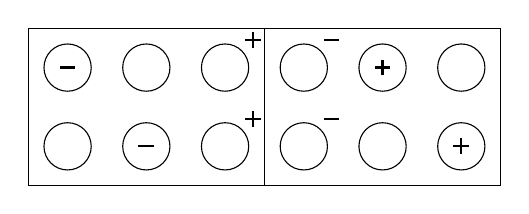
\begin{tikzpicture}
        %% rectangles
        \draw (0,0) rectangle (+3,2);
        \draw (0,0) rectangle (-3,2);
        %% circles
        \foreach \x in {-0.5,-1.5,-2.5,0.5,1.5,2.5}
            \foreach \y in {0.5,1.5}
                \draw (\x,\y) circle (0.3cm);
        %% negative charges
        \foreach \x/\y in {-2.5/1.5,-1.5/0.5,0.85/0.85,0.85/1.85}
            \foreach \z in {0,180}
                \draw[thick] (\x,\y) -- ++(\z:0.66ex);
        %% positive charges
        \foreach \x/\y in {1.5/1.5,2.5/0.5,-0.15/1.85,-0.15/0.85}
            \foreach \z in {0,90,180,270}
                \draw[thick] (\x,\y) -- ++(\z:0.66ex);
    \end{tikzpicture}
    \end{center}
    \begin{multicols}{2}
    \begin{choices}
        \wrongchoice{triode}
        \wrongchoice{transistor}
        \wrongchoice{donor}
      \correctchoice{diode}
    \end{choices}
    \end{multicols}
\end{question}
}

\element{nysed}{
\begin{question}{June1998-Q104}
    Indium is an element that has only three valence electrons.
    If a very small amount of indium was added to a germanium crystal,
        the resulting semiconductor would be:
    \begin{multicols}{2}
    \begin{choices}
        \wrongchoice{$N$-type}
      \correctchoice{$P$-type}
        \wrongchoice{negatively charged}
        \wrongchoice{positively charged}
    \end{choices}
    \end{multicols}
\end{question}
}

\element{nysed}{
\begin{question}{June1998-Q105}
    How should the junction of an $N$-$P$-$N$ transistor be biased?
    \begin{choices}
      \correctchoice{The emitter-base is forward biased and the base-collector is reverse biased}
        \wrongchoice{The emitter-base and collector-base are forward biased}
        \wrongchoice{The emitter-base is reverse biased and the base-collector is forward biased}
        \wrongchoice{The emitter-base and collector-base are reverse biased}
    \end{choices}
\end{question}
}


%% Section June1997
%%--------------------
\element{nysed}{
\begin{question}{June1997-Q96}
    Which graph best represents the relationship between conductivity and resistivity for a solid?
    \begin{multicols}{2}
    \begin{choices}
        \AMCboxDimensions{down=-2.5em}
        \wrongchoice{
            \begin{tikzpicture}
                \begin{axis}[
                    axis y line=left,
                    axis x line=bottom,
                    axis line style={->},
                    ylabel={resistivity},
                    ytick=\empty,
                    xlabel={conductivity},
                    xtick=\empty,
                    xmin=0,xmax=11,
                    ymin=0,ymax=11,
                    width=\columnwidth,
                    very thin,
                ]
                \addplot[line width=1pt,domain=0:10]{x};
                \end{axis}
            \end{tikzpicture}
        }
        %% ANS is B
        \correctchoice{
            \begin{tikzpicture}
                \begin{axis}[
                    axis y line=left,
                    axis x line=bottom,
                    axis line style={->},
                    ylabel={resistivity},
                    ytick=\empty,
                    xlabel={conductivity},
                    xtick=\empty,
                    xmin=0,xmax=11,
                    ymin=0,ymax=11,
                    width=\columnwidth,
                    very thin,
                ]
                \addplot[line width=1pt,domain=0:10]{10/x};
                \end{axis}
            \end{tikzpicture}
        }
        \wrongchoice{
            \begin{tikzpicture}
                \begin{axis}[
                    axis y line=left,
                    axis x line=bottom,
                    axis line style={->},
                    ylabel={resistivity},
                    ytick=\empty,
                    xlabel={conductivity},
                    xtick=\empty,
                    xmin=0,xmax=11,
                    ymin=0,ymax=11,
                    width=\columnwidth,
                    very thin,
                ]
                \addplot[line width=1pt,domain=0:10]{8};
                \end{axis}
            \end{tikzpicture}
        }
        \wrongchoice{
            \begin{tikzpicture}
                \begin{axis}[
                    axis y line=left,
                    axis x line=bottom,
                    axis line style={->},
                    ylabel={resistivity},
                    ytick=\empty,
                    xlabel={conductivity},
                    xtick=\empty,
                    xmin=0,xmax=11,
                    ymin=0,ymax=11,
                    width=\columnwidth,
                    very thin,
                ]
                \addplot[line width=1pt,domain=0:10]{0.1*x*x};
                \end{axis}
            \end{tikzpicture}
        }
    \end{choices}
    \end{multicols}
\end{question}
}

\element{nysed}{
\begin{question}{June1997-Q97}
    The diagram below shows an input of alternating current to
        a ``black box'' and the resulting output current.
    \begin{center}
    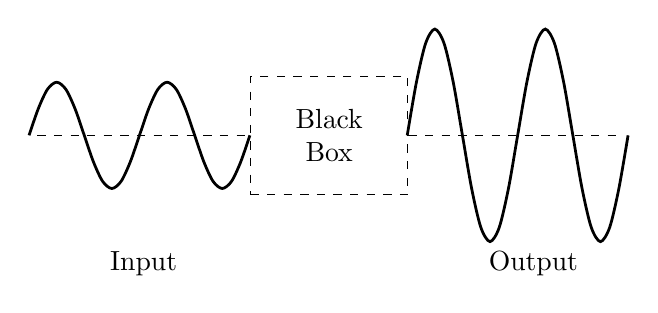
\begin{tikzpicture}[scale=0.9]
        %% black box
        \node[draw,dashed,anchor=west,minimum width=2cm,minimum height=1.5cm,text centered,text width=4em] (B) at (0,0) {Black Box};
        %% input
        \draw[dashed] (-3,0) -- (B.west);
        \draw[domain=0:4*pi,smooth,line width=1pt] plot ({-0.248*\x}, {-0.75*sin(\x r)});
        \node[anchor=north] at (-1.5,-1.5) {Input};
        %% output
        \draw[dashed] (B.east) -- ++(0:3);
        \draw[domain=0:4*pi,smooth,line width=1pt] plot ({2.22+0.248*\x}, {1.5*sin(\x r)});
        \node[anchor=north] at (+4,-1.5) {Output};
    \end{tikzpicture}
    \end{center}
    The ``black box'' most likely is:
    \begin{choices}
        \wrongchoice{an LED}
      \correctchoice{a transistor}
        \wrongchoice{a diode}
        \wrongchoice{an $N$-type semiconductor}
    \end{choices}
\end{question}
}

\element{nysed}{
\begin{question}{June1997-Q98}
    A $P$-type semiconductor is formed by adding impurities,
        which provide extra:
    \begin{multicols}{2}
    \begin{choices}
        \wrongchoice{electrons}
        \wrongchoice{protons}
        \wrongchoice{neutrons}
      \correctchoice{holes}
    \end{choices}
    \end{multicols}
\end{question}
}

\newcommand{\nysedJuneNineteenNinetySevenQNinetyNine}{
\ctikzset{bipoles/length=1.00cm}
\begin{circuitikz}
    %% battery
    \draw (0,0) to [battery] (6,0);
    \node[anchor=north east] at (2.8,0) {$+$};
    \node[anchor=north west] at (3.2,0) {$-$};
    \node[anchor=south east] at (2.8,0) {$A$};
    \node[anchor=south west] at (3.2,0) {$B$};
    %% circuit
    \draw (0,0) to (0,2) to (6,2) to (6,0);
    \node[draw,thick,minimum width=1cm,minimum height=0.5cm,fill=white,anchor=east] at (3,2) {$P$};
    \node[draw,thick,minimum width=1cm,minimum height=0.5cm,fill=white,anchor=west] at (3,2) {$N$};
\end{circuitikz}
}

\element{nysed}{
\begin{question}{June1997-Q99}
    The diagram below represents a semiconductor device connected to a battery.
    \begin{center}
        \nysedJuneNineteenNinetySevenQNinetyNine
    \end{center}
    In the circuit, holes migrate from:
    \begin{multicols}{2}
    \begin{choices}
        \wrongchoice{$A$ to $B$}
        \wrongchoice{$B$ to $A$}
        \wrongchoice{$N$ to $P$}
      \correctchoice{$P$ to $N$}
    \end{choices}
    \end{multicols}
\end{question}
}

\element{nysed}{
\begin{question}{June1997-Q100}
    The diagram below represents a semiconductor device connected to a battery.
    \begin{center}
        \nysedJuneNineteenNinetySevenQNinetyNine
    \end{center}
    If an alternating potential difference is substituted for the battery, the result will be:
    \begin{choices}
        \wrongchoice{an alternating current}
      \correctchoice{a pulsating direct current}
        \wrongchoice{a steady direct current}
        \wrongchoice{no current flow}
    \end{choices}
\end{question}
}

\element{nysed}{
\begin{question}{June1997-Q101}
    The diagram below represents a semiconductor device connected to a battery.
    \begin{center}
        \nysedJuneNineteenNinetySevenQNinetyNine
    \end{center}
    Which symbol best represents the orientation of the device shown in the circuit diagram?
    \begin{multicols}{2}
    \begin{choices}
        \AMCboxDimensions{down=-0.8cm}\small
        \ctikzset{bipoles/length=0.75cm}
        \wrongchoice{
            \begin{circuitikz}
                \draw[dashed,white!60!black] (-1.6,-1) rectangle (1.6,1);
                \node[pnp,rotate=90] (pnp) at (0,0) {};
                \draw (pnp.C) to (+1.5,0) node[anchor=south east] {Emitter};
                \draw (pnp.E) to (-1.5,0) node[anchor=south west] {Collector};
            \end{circuitikz}
        }
        \wrongchoice{
            \begin{circuitikz}
                \draw[dashed,white!60!black] (-1.6,-1) rectangle (1.6,1);
                \node[npn,rotate=270,xscale=-1] (npn) at (0,0) {};
                \draw (npn.E) to (-1.5,0) node[anchor=south west] {Collector};
                \draw (npn.C) to (+1.5,0) node[anchor=south east] {Emitter};
            \end{circuitikz}
        }
        \correctchoice{
            \begin{circuitikz}
                \draw[dashed,white!60!black] (-1.6,-1) rectangle (1.6,1);
                \draw (-1.5,0) to [thick,full diode] (1.5,0);
                \node[anchor=south west] at (-1.5,0) {Anode};
                \node[anchor=south east,xshift=1ex] at (+1.5,0) {Cathode};
            \end{circuitikz}
        }
        \wrongchoice{
            \begin{circuitikz}
                \draw[dashed,white!60!black] (-1.6,-1) rectangle (1.6,1);
                \draw (+1.5,0) to [thick,full diode] (-1.5,0);
                \node[anchor=south west] at (-1.5,0) {Anode};
                \node[anchor=south east,xshift=1ex] at (+1.5,0) {Cathode};
            \end{circuitikz}
        }
    \end{choices}
    \end{multicols}
\end{question}
}

\newcommand{\nysedJuneNineteenNInetySevenQOneHundredTwo}{
\ctikzset{bipoles/length=1.00cm}
\begin{circuitikz}
    %\draw (0,0) to [battery1,v=$ $] (3,0);
    \draw (0,0) to [battery,l=\SI{5}{\volt}] (3,0);
    \node[anchor=south east] at (1.4,0) {$-$};
    \node[anchor=south west] at (1.6,0) {$+$};
    \draw (0,0) to (0,2) to [thick,full diode] (3,2) to (3,0);
\end{circuitikz}
\begin{tikzpicture}
    %% NOTE: TODO: finish graph
    \begin{axis}[
        axis y line=middle,
        axis x line=middle,
        axis line style={->},
        ylabel={current},
        y unit=\si{\milli\ampere},
        ytick=\empty,
        xlabel={voltage},
        x unit=\si{\volt},
        xtick=\empty,
        xmin=0,xmax=11,
        ymin=0,ymax=11,
        width=\columnwidth,
        very thin,
    ]
    \addplot[line width=1pt,domain=-10:10]{0.1*x*x*x};
    \end{axis}
\end{tikzpicture}
}

\element{nysed}{
\begin{question}{June1997-Q102}
    \begin{center}
        \nysedJuneNineteenNInetySevenQOneHundredTwo
    \end{center}
    When connected as shown, the diode is:
    \begin{multicols}{2}
    \begin{choices}
      \correctchoice{forward biases}
        \wrongchoice{reverse biases}
        \wrongchoice{open biases}
        \wrongchoice{closed biases}
    \end{choices}
    \end{multicols}
\end{question}
}

\element{nysed}{
\begin{question}{June1997-Q103}
    \begin{center}
        \nysedJuneNineteenNInetySevenQOneHundredTwo
    \end{center}
    Compared to the voltage at which this diode avalanches,
        a more heavily doped diode would:
    \begin{choices}
      \correctchoice{avalanche at a lower voltage, only}
        \wrongchoice{avalanche at a higher voltage, only}
        \wrongchoice{not avalanche at any voltage}
        \wrongchoice{avalanche at any voltage}
    \end{choices}
\end{question}
}

\element{nysed}{
\begin{question}{June1997-Q104}
    The diagram below represents an operating transistor circuit.
    \begin{center}
    \ctikzset{bipoles/length=1.00cm}
    \begin{circuitikz}
        \draw (0,3) node[npn,rotate=270,xscale=-1] (npn) {}
            (npn.base) to [short,i=$I_b$] (0,0) to (2,0) to [battery,l=$V_{bc}$] (2,3);
        \draw (npn.emitter) to (-2,3) to [battery1,l=$V_{eb}$] (-2,0) to (0,0);
        \draw (npn.collector) to [short,i=$I_e$] (2,3);
        \draw (-2,3) to [short,i=$I_e$] (npn.emitter);
    \end{circuitikz}
    \end{center}
    Which currents are approximately equal?
    \begin{multicols}{2}
    \begin{choices}
        \wrongchoice{$I_b$ and $I_e$, only}
        \wrongchoice{$I_b$ and $I_c$, only}
      \correctchoice{$I_c$ and $I_e$, only}
        \wrongchoice{$I_b$, $I_c$, and $I_e$}
    \end{choices}
    \end{multicols}
\end{question}
}

\element{nysed}{
\begin{question}{June1997-Q105}
    A student measures a current of \SI{0.05}{\ampere} through a $P$-type semiconductor.
    If the battery connections are reversed,
        the current through the semiconductor will be:
    \begin{choices}
        \wrongchoice{less than \SI{0.05}{\ampere}}
        \wrongchoice{greater than \SI{0.05}{\ampere}}
      \correctchoice{equal to \SI{0.05}{\ampere}}
    \end{choices}
\end{question}
}


%% Section June1996
%%--------------------
\element{nysed}{
\begin{question}{June1996-Q96}
    Copper is to conductor as germanium is to:
    \begin{multicols}{2}
    \begin{choices}
        \wrongchoice{insulator}
        \wrongchoice{fuse}
        \wrongchoice{resistor}
      \correctchoice{semiconductor}
    \end{choices}
    \end{multicols}
\end{question}
}

\element{nysed}{
\begin{question}{June1996-Q97}
    The diagram at the right shows the valence and conduction bands of an intrinsic semiconductor.
    Some of the electrons in the valence band have been promoted to the conduction band.
    \begin{center}
    \begin{tikzpicture}
        %% conduction band
        \begin{scope}[yshift=+1.5cm]
            \draw (-1,0) rectangle (1,2);
            \draw[pattern=north east lines] (-1,0) rectangle (1,0.5);
            \node[text width=10em,anchor=south west,font=\small] (A) at (1,0.75) {Electrons ($-$) promoted to conduction band};
            \draw[->] (A.south) |- (1,0.25);
            \node[anchor=south] at (0,2) {Conduction Band};
        \end{scope}
        %% valence band
        \begin{scope}[yshift=-1.5cm]
            \draw (-1,0) rectangle (1,2);
            \draw[pattern=north east lines] (-1,0) rectangle (1,1.5);
            \node[text width=6em,anchor=north west,font=\small] (A) at (1,1.5) {Deficiency of electrons (holes)};
            \draw[->] (A.north) |- (1,1.75);
            \node[anchor=north] at (0,0) {Valence Band};
        \end{scope}
    \end{tikzpicture}
    \end{center}
    Which diagram below best represents the valence and conduction bands of the intrinsic semiconductor when its temperature is increased?
    \begin{multicols}{2}
    \begin{choices}
        \AMCboxDimensions{down=-2.0cm}
        \wrongchoice{
            \begin{tikzpicture}
                \draw[dashed,white!60!black] (-1.25,-1.25) rectangle (1.25,3.25);
                \begin{scope}[yshift=+1.1cm]
                    \draw (-1,0) rectangle (1,2);
                    \draw[pattern=north east lines] (-1,0) rectangle (1,0.05);
                \end{scope}
                \begin{scope}[yshift=-1.1cm]
                    \draw (-1,0) rectangle (1,2);
                    \draw[pattern=north east lines] (-1,0) rectangle (1,1.95);
                \end{scope}
            \end{tikzpicture}
        }
        \wrongchoice{
            \begin{tikzpicture}
                \draw[dashed,white!60!black] (-1.25,-1.25) rectangle (1.25,3.25);
                \begin{scope}[yshift=+1.1cm]
                    \draw (-1,0) rectangle (1,2);
                    \draw[pattern=north east lines] (-1,0) rectangle (1,0.1);
                \end{scope}
                \begin{scope}[yshift=-1.1cm]
                    \draw (-1,0) rectangle (1,2);
                    \draw[pattern=north east lines] (-1,0) rectangle (1,1.9);
                \end{scope}
            \end{tikzpicture}
        }
        %% ANS is 3
        \correctchoice{
            \begin{tikzpicture}
                \draw[dashed,white!60!black] (-1.25,-1.25) rectangle (1.25,3.25);
                \begin{scope}[yshift=+1.1cm]
                    \draw (-1,0) rectangle (1,2);
                    \draw[pattern=north east lines] (-1,0) rectangle (1,0.5);
                \end{scope}
                \begin{scope}[yshift=-1.1cm]
                    \draw (-1,0) rectangle (1,2);
                    \draw[pattern=north east lines] (-1,0) rectangle (1,1.5);
                \end{scope}
            \end{tikzpicture}
        }
        \wrongchoice{
            \begin{tikzpicture}
                \draw[dashed,white!60!black] (-1.25,-1.25) rectangle (1.25,3.25);
                \begin{scope}[yshift=+1.1cm]
                    \draw[pattern=north east lines] (-1,0) rectangle (1,2);
                \end{scope}
                \begin{scope}[yshift=-1.1cm]
                    \draw[pattern=north east lines] (-1,0) rectangle (1,2);
                \end{scope}
            \end{tikzpicture}
        }
    \end{choices}
    \end{multicols}
\end{question}
}

\element{nysed}{
\begin{question}{June1996-Q98}
    What does the diagram below represent?
    \begin{center}
    \ctikzset{bipoles/length=0.75cm}
    \begin{circuitikz}
        \node[npn,rotate=270,xscale=-1] (npn) at (0,0) {};
        \draw (npn.C) to (+2,0) node[anchor=south east] {Collector};
        \draw (npn.E) to (-2,0) node[anchor=south west] {Emitter};
        \draw (npn.B) to (0,-1) node[anchor=south west] {Base};
    \end{circuitikz}
    \end{center}
    \begin{multicols}{2}
    \begin{choices}
      \correctchoice{an $N$-$P$-$N$ transitor}
        \wrongchoice{an $P$-$N$-$P$ transitor}
        \wrongchoice{an zener diode}
        \wrongchoice{an avalanche region}
    \end{choices}
    \end{multicols}
\end{question}
}

\newcommand{\nysedJuneNinteenNinetySixQNinetyNine}{
\ctikzset{bipoles/length=1.00cm}
\begin{circuitikz}
    \draw (0,0) to [battery] (6,0) to (6,2) to  (0,2) to (0,0);
    \node[draw,fill=white,anchor=center,text centered,text width=6em] (N) at (3,2) {$N$-type semiconductor};
    \fill (N.west) circle (2pt) node[anchor=south east] {$A$};
    \fill (N.east) circle (2pt) node[anchor=south west] {$B$};
    \fill (0,1) circle (2pt) node[anchor=east] {$C$};
    \node[anchor=south west] at (3.2,0) {$+$};
    \node[anchor=south east] at (2.8,0) {$-$};
\end{circuitikz}
}

\element{nysed}{
\begin{question}{June1996-Q99}
    The diagram below represents an $N$-type silicon semiconductor connected to a battery.
    \begin{center}
        \nysedJuneNinteenNinetySixQNinetyNine
    \end{center}
    A very small amount of antimony which has 5 valence electrons,
        had previously been added to the silicon crystal.
    This process produced:
    \begin{choices}
      \correctchoice{an excess of free electrons}
        \wrongchoice{an excess of free protons}
        \wrongchoice{more resistance}
        \wrongchoice{a higher emf}
    \end{choices}
\end{question}
}

\element{nysed}{
\begin{question}{June1996-Q100}
    The diagram below represents an $N$-type silicon semiconductor connected to a battery.
    \begin{center}
        \nysedJuneNinteenNinetySixQNinetyNine
    \end{center}
    Which statement best describes the flow of charge through the conducting wire between points $A$ and $C$?
    \begin{choices}
        \wrongchoice{Electrons flow from $A$ to $C$}
      \correctchoice{Electrons flow from $C$ to $A$}
        \wrongchoice{Holes flow from $A$ to $C$}
        \wrongchoice{Holes flow from $C$ to $A$}
    \end{choices}
\end{question}
}

\element{nysed}{
\begin{question}{June1996-Q101}
    Which diagram below represents a $P$-$N$ junction with a forward bias?
    \begin{multicols}{2}
    \begin{choices}
        \AMCboxDimensions{down=-0.8cm}
        %% ANS is 1
        \correctchoice{
            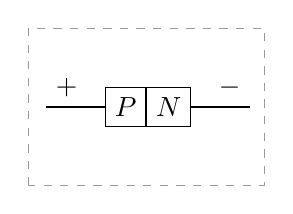
\begin{tikzpicture}
                \draw[dashed,white!60!black] (-1.5,-1) rectangle (1.5,1);
                \node[anchor=east,draw,minimum size=0.5cm] (P) at (0,0) {$P$};
                \node[anchor=west,draw,minimum size=0.5cm] (N) at (0,0) {$N$};
                \draw (P.west) -- ++(180:0.75) node[anchor=south west] {$+$};
                \draw (N.east) -- ++(0:0.75) node[anchor=south east] {$-$};
            \end{tikzpicture}
        }
        \wrongchoice{
            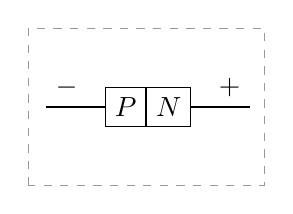
\begin{tikzpicture}
                \draw[dashed,white!60!black] (-1.5,-1) rectangle (1.5,1);
                \node[anchor=east,draw,minimum size=0.5cm] (P) at (0,0) {$P$};
                \node[anchor=west,draw,minimum size=0.5cm] (N) at (0,0) {$N$};
                \draw (P.west) -- ++(180:0.75) node[anchor=south west] {$-$};
                \draw (N.east) -- ++(0:0.75) node[anchor=south east] {$+$};
            \end{tikzpicture}
        }
        \wrongchoice{
            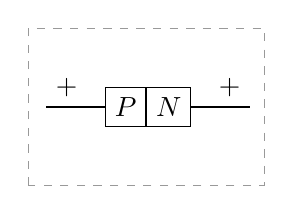
\begin{tikzpicture}
                \draw[dashed,white!60!black] (-1.5,-1) rectangle (1.5,1);
                \node[anchor=east,draw,minimum size=0.5cm] (P) at (0,0) {$P$};
                \node[anchor=west,draw,minimum size=0.5cm] (N) at (0,0) {$N$};
                \draw (P.west) -- ++(180:0.75) node[anchor=south west] {$+$};
                \draw (N.east) -- ++(0:0.75) node[anchor=south east] {$+$};
            \end{tikzpicture}
        }
        \wrongchoice{
            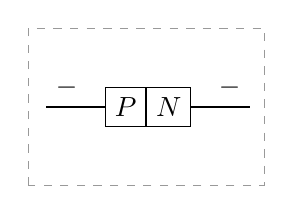
\begin{tikzpicture}
                \draw[dashed,white!60!black] (-1.5,-1) rectangle (1.5,1);
                \node[anchor=east,draw,minimum size=0.5cm] (P) at (0,0) {$P$};
                \node[anchor=west,draw,minimum size=0.5cm] (N) at (0,0) {$N$};
                \draw (P.west) -- ++(180:0.75) node[anchor=south west] {$-$};
                \draw (N.east) -- ++(0:0.75) node[anchor=south east] {$-$};
            \end{tikzpicture}
        }
    \end{choices}
    \end{multicols}
\end{question}
}

\element{nysed}{
\begin{question}{June1996-Q102}
    Materials such as indium that provide ``holes'' to semiconductors are often referred to as:
    \begin{multicols}{2}
    \begin{choices}
        \wrongchoice{holistic}
        \wrongchoice{donors}
      \correctchoice{acceptors}
        \wrongchoice{$N$-types}
    \end{choices}
    \end{multicols}
\end{question}
}

\element{nysed}{
\begin{question}{June1996-Q103}
    The diagram below shows alternating current input to a black box containing diodes.
    \begin{center}
    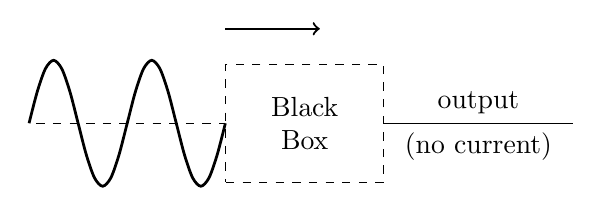
\begin{tikzpicture}[scale=0.8]
        %% black box
        \node[draw,dashed,anchor=west,minimum width=2cm,minimum height=1.5cm,text centered,text width=4em] (B) at (0,0) {Black Box};
        \draw[thick,->] (0,1.5) -- (1.5,1.5);
        %% input
        \draw[dashed] (-3,0) -- (B.west);
        \draw[domain=0:4*pi,smooth,line width=1pt] plot ({-0.248*\x}, {-1*sin(\x r)});
        %% output
        \draw (B.east) -- ++(0:3)
            node[pos=0.5,anchor=south] {output}
            node[pos=0.5,anchor=north] {(no current)};
    \end{tikzpicture}
    \end{center}
    Which diode configuration in the black box accounts for the output (no current)?
    \begin{multicols}{2}
    \begin{choices}
        \AMCboxDimensions{down=-0.8cm}
        \ctikzset{bipoles/length=0.75cm}
        \wrongchoice{
            \begin{circuitikz}
                \draw[dashed,white!60!black] (-1.5,-1) rectangle (1.5,1);
                \draw[thick,->] (-1.5,1.25) -- (0,1.25);
                \draw (-1.5,0) to [full diode] (0,0) to [full diode] (1.5,0);
            \end{circuitikz}
        }
        \correctchoice{
            \begin{circuitikz}
                \draw[dashed,white!60!black] (-1.5,-1) rectangle (1.5,1);
                \draw[thick,->] (-1.5,1.25) -- (0,1.25);
                \draw (-1.5,0) to [full diode] (0,0);
                \draw (+1.5,0) to [full diode] (0,0);
            \end{circuitikz}
        }
        \wrongchoice{
            \begin{circuitikz}
                \draw[dashed,white!60!black] (-1.5,-1) rectangle (1.5,1);
                \draw[thick,->] (-1.5,1.25) -- (0,1.25);
                \draw (-1.5,0) to (-1,0) to (-1,0.5) to [full diode] (1,0.5) to (1,0) to (1.5,0);
                \draw (+1,0) to (+1,-0.5) to [full diode] (-1,-0.5) to (-1,0);
            \end{circuitikz}
        }
        \wrongchoice{
            \begin{circuitikz}
                \draw[dashed,white!60!black] (-1.5,-1) rectangle (1.5,1);
                \draw[thick,->] (-1.5,1.25) -- (0,1.25);
                \draw (-1.5,0) to [full diode] (1.5,0);
            \end{circuitikz}
        }
    \end{choices}
    \end{multicols}
\end{question}
}

\element{nysed}{
\begin{question}{June1996-Q104}
    As a result of transistor amplitification,
        small increases in the emitter-base current will bring about large:
    \begin{choices}
        \wrongchoice{decreases in the emitter-base voltage}
        \wrongchoice{decreases in the collector current}
        \wrongchoice{increases in the emitter-base voltage}
      \correctchoice{increases in the collector current}
    \end{choices}
\end{question}
}

\element{nysed}{
\begin{question}{June1996-Q105}
    A source of alternating current, a junction diode, and a lamp are connected, as shown in the diagram below.
    \begin{center}
    \ctikzset{bipoles/length=1.00cm}
    \begin{circuitikz}
        \draw (0,0) to [sV,l={a.c. source}] (0,3) to [full diode,l={Diode}] (3,3) to [R,l={lamp}] (3,0) to (0,0);
    \end{circuitikz}
    \end{center}
    The current passing through the lamp is:
    \begin{choices}
        \wrongchoice{alternating current, only}
      \correctchoice{direct current, only}
        \wrongchoice{both alternating and direct current}
    \end{choices}
\end{question}
}


%% Section June1995
%%--------------------
\element{nysed}{
\begin{question}{June1995-Q96}
    The circuit diagram below shows a $P$-type semiconductor in series with a lamp,
        a resistor, and a battery.
    \begin{center}
    \ctikzset{bipoles/length=0.75cm}
    \begin{circuitikz}
        \draw (0,0) to (3,0) to (7,0) to (7,2) to [R,l=$R$] (5,2) to [european resistor,l={Lamp}] (3,2) to (0,2) to (0,0);
        \draw (3,0) to [battery1,v=$ $] (0,0);
        \node[anchor=center,draw,fill=white,text width=6em,text centered] at (1.5,2) {$P$-type semiconductor};
    \end{circuitikz}
    \end{center}
    What would increase the current in the circuit?
    \begin{choices}
        \wrongchoice{increasing the resistance of the resistor}
        \wrongchoice{reversing the battery polarity}
        \wrongchoice{reversing the connections to the semiconductor}
      \correctchoice{increasing the temperature of the semiconductor}
    \end{choices}
\end{question}
}

\element{nysed}{
\begin{question}{June1995-Q97}
    According to the energy band model,
        in which material is the energy gap between the conduction band and the valence band greatest?
    \begin{choices}
        \wrongchoice{a conductor}
      \correctchoice{an insulator}
        \wrongchoice{an extrinsic semiconductor}
        \wrongchoice{an intrinsic semiconductor}
    \end{choices}
\end{question}
}

\element{nysed}{
\begin{question}{June1995-Q98}
    The diagram below shows a circuit connecting a battery to a semiconductor $A$.
    \begin{center}
    \ctikzset{bipoles/length=0.75cm}
    \begin{circuitikz}
        \draw (0,0) to (3,0) to (6,0) to (6,2) to (0,2) to (0,0);
        \draw (3,0) to [battery,v=$ $] (0,0);
        \node[anchor=center,draw,minimum width=2cm,minimum height=1cm,fill=white] at (2,2) {};
        \node[anchor=center,draw,minimum width=2cm,minimum height=1cm,pattern=north east lines] at (2,2) {};
        \node[anchor=center,fill=white] at (2,2) {$A$};
    \end{circuitikz}
    \end{center}
    If the battery connection is reverse,
        the current in the circuit will:
    \begin{choices}
        \wrongchoice{decrease only if $A$ is $N$-type}
        \wrongchoice{decrease only if $A$ is $P$-type}
        \wrongchoice{increase if $A$ is either $A$ is $N$-type or $P$-type}
      \correctchoice{remain the same is $A$ is either $N$-type or $P$-type}
    \end{choices}
\end{question}
}

\element{nysed}{
\begin{question}{June1995-Q99}
    The majority charge carriers in a $P$-type semiconductor are holes.
    When a section of $P$-type semiconductor is connected across the terminal of a battery,
        where do the holes flow?
    \begin{choices}
      \correctchoice{toward the negative terminal, only}
        \wrongchoice{toward the positive terminal, only}
        \wrongchoice{equally toward both the negative and positive terminals}
        \wrongchoice{toward neither terminal}
    \end{choices}
\end{question}
}

\element{nysed}{
\begin{question}{June1995-Q100}
    The simplest circuit element that will allow electric current to pass through a circuit in only one direction is:
    \begin{choices}
        \wrongchoice{a transistor}
      \correctchoice{a diode}
        \wrongchoice{an $N$-type semiconductor}
        \wrongchoice{a $P$-type semiconductor}
    \end{choices}
\end{question}
}

\element{nysed}{
\begin{question}{June1995-Q101}
    The graph below shows the relationship between current and applied potential difference for an electrical device.
    \begin{center}
    \begin{tikzpicture}
        \begin{axis}[
            axis y line=left,
            axis x line=bottom,
            axis line style={->},
            xlabel={potential},
            xtick={5},
            xticklabels={\SI{1.0}{\volt}},
            x label style={
                at={(axis cs:4,0)},
                anchor=north east,
            },
            ylabel={current},
            ytick=\empty,
            xmin=0,xmax=6,
            ymin=0,ymax=10,
            width=1.0\columnwidth,
            height=0.618\columnwidth,
            very thin,
        ]
        \addplot[line width=1pt,domain=0:5] {-1 + 1/(1-(x/5)^2)};
        \draw[dashed] (axis cs:5,0) -- (axis cs:5,10);
        \end{axis}
    \end{tikzpicture}
    \end{center}
    This device is most likely a:
    \begin{choices}
        \wrongchoice{forward-biased $P$-type semiconductor}
        \wrongchoice{reverse-biased $P$-type semiconductor}
      \correctchoice{forward-biased $P$-$N$ junction}
        \wrongchoice{reverse-biased $P$-$N$ junction}
    \end{choices}
\end{question}
}

\element{nysed}{
\begin{question}{June1995-Q102}
    \ctikzset{bipoles/length=0.5cm}
    The symbol \tikz \draw (0,0) to [diode] (0.5,0); is to a $P$-$N$ junction as the symbol \tikz \node[pnp,rotate=90,scale=0.5] at (0,0) {}; is to:
    \begin{choices}
        \wrongchoice{an $N$-$P$-$N$ transistor}
      \correctchoice{a $P$-$N$-$P$ transistor}
        \wrongchoice{a zener diode}
        \wrongchoice{an integrated circuit}
    \end{choices}
\end{question}
}

\element{nysed}{
\begin{question}{June1995-Q103}
    The diagram below shows an $N$-$P$-$N$ semiconductor device.
    \begin{center}
    \ctikzset{bipoles/length=0.75cm}
    \begin{circuitikz}
        \draw (6,0) to [battery,v=$ $] (0,0) to (0,2) to (6,2) to (6,0);
        \node[anchor=center,draw,minimum size=1cm,fill=white] (P) at (3,2) {$P$};
        \node[anchor=east,draw,minimum size=1cm,fill=white] at (P.west) {$N$};
        \node[anchor=west,draw,minimum size=1cm,fill=white] at (P.east) {$N$};
    \end{circuitikz}
    \end{center}
    The base in the semiconductor shown is the:
    \begin{multicols}{2}
    \begin{choices}
        \wrongchoice{right $N$}
        \wrongchoice{left $N$}
      \correctchoice{$P$}
        \wrongchoice{$P$-$N$ junction}
    \end{choices}
    \end{multicols}
\end{question}
}

\element{nysed}{
\begin{question}{June1995-Q104}
    A student is designing a circuit to amplify a small voltage change into a larger voltage change.
    The electric circuit element best suited to this task is:
    \begin{choices}
      \correctchoice{a transistor}
        \wrongchoice{a diode}
        \wrongchoice{an $N$-type semiconductor}
        \wrongchoice{a $P$-type semiconductor}
    \end{choices}
\end{question}
}

\element{nysed}{
\begin{question}{June1995-Q105}
    What is the name for a large group of electronic components that are interconnected on a single block of silicon inside a computer?
    \begin{choices}
        \wrongchoice{a thermistor}
      \correctchoice{an integrated circuit}
        \wrongchoice{a transistor}
        \wrongchoice{a collector}
    \end{choices}
\end{question}
}


%% Section June1994
%%--------------------
\element{nysed}{
\begin{question}{June1994-Q96}
    Which quantity is equal to the reciprocal of resistivity?
    \begin{multicols}{2}
    \begin{choices}
      \correctchoice{conductivity}
        \wrongchoice{current}
        \wrongchoice{resistance}
        \wrongchoice{voltage}
    \end{choices}
    \end{multicols}
\end{question}
}

\element{nysed}{
\begin{question}{June1994-Q97}
    A solid is determined to be a conductor,
        an insulator, or a semiconductor on the basis of:
    \begin{choices}
        \wrongchoice{its melting point and boiling point}
        \wrongchoice{its atomic number and mass number}
      \correctchoice{the number of electrons in the conduction band and the energy gap between bands}
        \wrongchoice{the number of electrons per squared meter of cross-sectional area of the material}
    \end{choices}
\end{question}
}

\element{nysed}{
\begin{question}{June1994-Q98}
    $P$-type semiconducting material functions primarily as:
    \begin{choices}
        \wrongchoice{an acceptor of protons}
      \correctchoice{an acceptor of electrons}
        \wrongchoice{a donor of protons}
        \wrongchoice{a donor of electrons}
    \end{choices}
\end{question}
}

\element{nysed}{
\begin{question}{June1994-Q99}
    What permits current to flow through a semiconductor when it is connected to a battery,
        as shown in the diagram.
    \begin{center}
    \ctikzset{bipoles/length=1.00cm}
    \begin{circuitikz}
        \draw (4,0) to  [battery,v_=$ $] (0,0) to (0,2) to (4,2) to (4,0);
        \node[draw,thick,anchor=center,minimum height=1cm,fill=white] at (2,2) {\small Semiconductor};
    \end{circuitikz}
    \end{center}
    \begin{choices}
        \wrongchoice{holes moving toward the right, only}
        \wrongchoice{electrons moving toward the left, only}
        \wrongchoice{both electrons and holes moving toward the left}
      \correctchoice{electrons moving left and holes moving right}
    \end{choices}
\end{question}
}

\element{nysed}{
\begin{question}{June1994-Q100}
    The diagram below shows the alternating current input signal to a diode.
    \begin{center}
    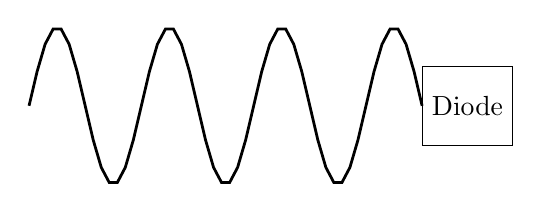
\begin{tikzpicture}
        %% diode
        \node[draw,minimum size=1cm,anchor=west] at (0,0) {Diode};
        %% input
        \begin{scope}[x=0.227cm]
            \draw[line width=1pt,domain=0:7*pi,samples=50] plot (-\x, {sin(\x r)});
        \end{scope}
    \end{tikzpicture}
    \end{center}
    Which diagram below best represents the output signal?
    \begin{multicols}{2}
    \begin{choices}
        \AMCboxDimensions{down=-1.2cm}
        \wrongchoice{
            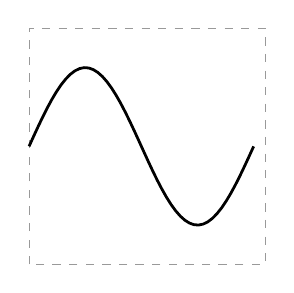
\begin{tikzpicture}
                \draw[dashed,white!60!black] (0,-1.5) rectangle (3,1.5);
                \begin{scope}[x=0.454cm]
                    \draw[line width=1pt,domain=0:2*pi,samples=50] plot (\x, {sin(\x r)});
                \end{scope}
            \end{tikzpicture}
        }
        %% ANS is 2
        \correctchoice{
            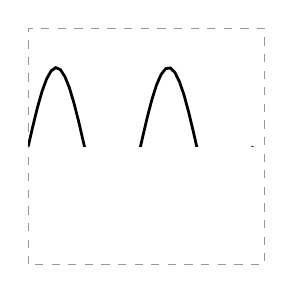
\begin{tikzpicture}
                \draw[dashed,white!60!black] (0,-1.5) rectangle (3,1.5);
                \clip (0,0) rectangle (3,1.5);
                \begin{scope}[x=0.227cm]
                    \draw[line width=1pt,domain=0:4*pi,samples=50] plot (\x, {sin(\x r)});
                \end{scope}
            \end{tikzpicture}
        }
        \wrongchoice{
            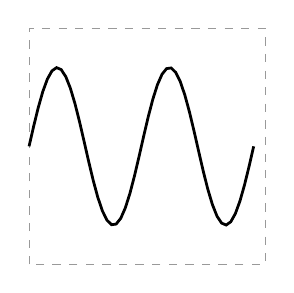
\begin{tikzpicture}
                \draw[dashed,white!60!black] (0,-1.5) rectangle (3,1.5);
                \begin{scope}[x=0.227cm]
                    \draw[line width=1pt,domain=0:4*pi,samples=50] plot (\x, {sin(\x r)});
                \end{scope}
            \end{tikzpicture}
        }
        \wrongchoice{
            \begin{tikzpicture}
                \draw[dashed,white!60!black] (0,-1.5) rectangle (3,1.5);
                \clip (0,0) rectangle (3,1.5);
                \begin{scope}[x=0.454cm]
                    \draw[line width=1pt,domain=0:2*pi,samples=50] plot (\x, {sin(\x r)});
                \end{scope}
            \end{tikzpicture}
        }
    \end{choices}
    \end{multicols}
\end{question}
}

\element{nysed}{
\begin{question}{June1994-Q101}
    What is a basic difference between a transistor and a diode?
    \begin{choices}
      \correctchoice{the number of junctions between $P$-type and $N$-type material}
        \wrongchoice{the size of the single junction between th $P$-type and $N$-type material}
        \wrongchoice{the nature of the donor material used in the $N$-type semiconductor}
        \wrongchoice{the amount of current applied to the semiconductor material}
    \end{choices}
\end{question}
}

\element{nysed}{
\begin{question}{June1994-Q102}
    In the diagram below, which part of the operating $N$-$P$-$N$ transistor is the collector?
    \begin{center}
    \ctikzset{bipoles/length=1.00cm}
    \begin{circuitikz}
        %% left
        \draw (0,0) to (-3,0) to (-3,3) to (0,3) to (0,0);
        \draw (-3,0) to [battery,v=$ $] (0,0);
        %% right
        \draw (0,0) to (+3,0) to (+3,3) to (0,3) to (0,0);
        \draw (0,0) to [battery,v=$ $] (3,0);
        %% NPN
        \node[draw,minimum size=1cm,fill=white,anchor=center] (P) at (0,3) {$P$};
        \node[draw,minimum size=1cm,fill=white,anchor=east] at (P.west) {$N$};
        \node[draw,minimum size=1cm,fill=white,anchor=west] at (P.east) {$N$};
    \end{circuitikz}
    \end{center}
    \begin{choices}
        \wrongchoice{the left $N$-type section}
      \correctchoice{the right $N$-type section}
        \wrongchoice{the left $P$-$N$  junction}
        \wrongchoice{the right $P$-$N$ junction}
    \end{choices}
\end{question}
}

\element{nysed}{
\begin{question}{June1994-Q103}
    A small change in the emitter-base current in a transistor brings about a large change in the collector current.
    This current-increasing property of a transistor is called:
    \begin{multicols}{2}
    \begin{choices}
      \correctchoice{amplification}
        \wrongchoice{biasing}
        \wrongchoice{Ohm's law}
        \wrongchoice{rectification}
    \end{choices}
    \end{multicols}
\end{question}
}

\element{nysed}{
\begin{question}{June1994-Q104}
    The graph below shows current verse potential difference for a diode.
    \begin{center}
    \begin{tikzpicture}
        \begin{axis}[
            axis y line=middle,
            axis x line=middle,
            axis line style={->},
            xlabel={potential},
            x unit=\si{\volt},
            xtick={5},
            xticklabels={0.7},
            x label style={
                at={(axis cs:5,-4)},
                anchor=north,
            },
            ylabel={current},
            y unit=\si{\milli\ampere},
            ytick=\empty,
            y label style={
                anchor=north east,
            },
            xmin=-10,xmax=7,
            ymin=-10,ymax=10,
            width=1.0\columnwidth,
            height=0.618\columnwidth,
            very thin,
        ]
        \addplot[line width=1pt,domain=0:5] {-1 + 1/(1-(x/5)^2)};
        \addplot[line width=1pt,domain=-10:0] {+1 - 1/(1-(x/10)^2)};
        \draw[dashed] (axis cs:5,0) -- (axis cs:5,10);
        \node[pin={[pin distance=4ex,pin edge={-latex},text centered,text width=4em]340:Avalanche Region}] at (axis cs:-9,-3) {};
        \end{axis}
    \end{tikzpicture}
    \end{center}
    The ``avalanche'' occurs only if the diode circuit is:
    \begin{multicols}{2}
    \begin{choices}
        \wrongchoice{open}
        \wrongchoice{closed}
      \correctchoice{reverse biased}
        \wrongchoice{forward biased}
    \end{choices}
    \end{multicols}
\end{question}
}

\element{nysed}{
\begin{question}{June1994-Q105}
    As the amount of doping material in the semiconductor increases,
        the magnitude of the voltage required for the ``avalanche'' to occur:
    \begin{choices}
      \correctchoice{decreases}
        \wrongchoice{increases}
        \wrongchoice{remains the same}
    \end{choices}
\end{question}
}


%% Section June1990
%%--------------------
\element{nysed}{
\begin{question}{June1990-Q101}
    According to accepted atomic models,
        metal are good conductors because their atoms have:
    \begin{choices}
        \wrongchoice{more electrons than protons}
        \wrongchoice{unstable nuclei that emit electrons}
        \wrongchoice{negative electrons that are attracted to positive protons}
      \correctchoice{a number of valence electrons that can move easily}
    \end{choices}
\end{question}
}

\element{nysed}{
\begin{question}{June1990-Q102}
    What type of semiconductor is represented by the diagram?
    \begin{center}
    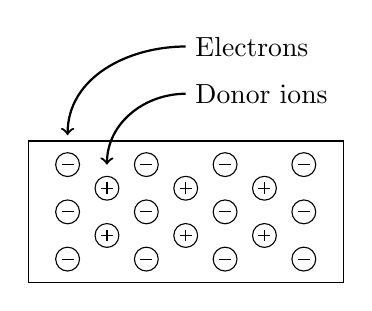
\begin{tikzpicture}
        \def\w{5}\def\h{3}
        \draw (0,0) rectangle ({\w*8 mm},{\h*6mm});
        %% labels
        \node[anchor=west] (A) at ({0.5*\w*8 mm},{(\h +2)*6mm}) {Electrons};
        \node[anchor=west] (B) at ({0.5*\w*8 mm},{(\h +1)*6mm}) {Donor ions};
        \draw[thick,->] (A.west) to[out=180,in=90] ({\w*1 mm},{1.25*\h*5 mm});
        \draw[thick,->] (B.west) to[out=180,in=90] ({\w*2 mm},{1.25*\h*4 mm});
        %% Electrons
        \foreach \x in {1,3,5,7}
            \foreach \y in {1,3,5} {
                \draw ({\w*\x mm},{\h*\y mm}) circle (1ex);
                \foreach \z in {0,180}
                    \draw ({\w*\x mm},{\h*\y mm}) -- ++(\z:0.5ex);
            }
        %% Donor ions
        \foreach \x in {2,4,6}
            \foreach \y in {2,4} {
                \draw ({\w*\x mm},{\h*\y mm}) circle (1ex);
                \foreach \z in {0,90,180,270}
                    \draw ({\w*\x mm},{\h*\y mm}) -- ++(\z:0.5ex);
            }
    \end{tikzpicture}
    \end{center}
    \begin{multicols}{2}
    \begin{choices}
        \wrongchoice{$P$-type}
      \correctchoice{$N$-type}
        \wrongchoice{$N$-$P$-type}
        \wrongchoice{$P$-$N$-type}
    \end{choices}
    \end{multicols}
\end{question}
}

\element{nysed}{
\begin{question}{June1990-Q103}
    Which device could be used to amplify the input signal in a microphone-speaker circuit?
    \begin{multicols}{2}
    \begin{choices}
        \wrongchoice{diode}
        \wrongchoice{resistor}
      \correctchoice{transistor}
        \wrongchoice{solenoid}
    \end{choices}
    \end{multicols}
\end{question}
}

\element{nysed}{
\begin{question}{June1990-Q104}
    Which diagram below correctly represents the basic operating circuit of an $N$-$P$-$N$ transistor?
    \begin{multicols}{2}
    \begin{choices}[o]
        \ctikzset{bipoles/length=0.75cm}
        \AMCboxDimensions{down=-2.5em}
        %% ANS is 1
        \correctchoice{
            \begin{circuitikz}[xscale=0.66]
                %% circuit
                \node[npn,rotate=270,xscale=-1] (npn) at (0,3) {};
                \draw (npn.E) to (-2,3) to [battery1,l=$V_E$] (-2,0) to (0,0);
                \draw (npn.B) to (0,0) to (2,0) to [battery,l=$V_c$] (2,1.5) to [R,l=$R$] (2,3) to (npn.C);
                %% labels
                \node[anchor=south east] at (-0.33,3) {$E$};
                \node[anchor=south west] at (+0.33,3) {$C$};
                \node[anchor=north west] at (0,2.33) {$B$};
            \end{circuitikz}
        }
        \wrongchoice{
            \begin{circuitikz}[xscale=0.66]
                \node[npn,rotate=90] (npn) at (0,3) {};
                \draw (npn.C) to (-2,3) to [battery1,l=$V_E$] (-2,0) to (0,0);
                \draw (npn.B) to (0,0) to (2,0) to [battery,l=$V_c$] (2,1.5) to [R,l=$R$] (2,3) to (npn.E);
                %% labels
                \node[anchor=south east] at (-0.33,3) {$E$};
                \node[anchor=south west] at (+0.33,3) {$C$};
                \node[anchor=north west] at (0,2.33) {$B$};
            \end{circuitikz}
        }
        \wrongchoice{
            \begin{circuitikz}[xscale=0.66]
                \node[pnp,rotate=90] (pnp) at (0,3) {};
                \draw (pnp.E) to (-2,3) to [battery1,l=$V_E$] (-2,0) to (0,0);
                \draw (pnp.B) to (0,0) to (2,0) to [battery,l=$V_c$] (2,1.5) to [R,l=$R$] (2,3) to (pnp.C);
                %% labels
                \node[anchor=south east] at (-0.33,3) {$E$};
                \node[anchor=south west] at (+0.33,3) {$C$};
                \node[anchor=north west] at (0,2.33) {$B$};
            \end{circuitikz}
        }
        \wrongchoice{
            \begin{circuitikz}[xscale=0.66]
                \node[pnp,rotate=270,xscale=-1] (pnp) at (0,3) {};
                \draw (pnp.C) to (-2,3) to [battery1,l=$V_E$] (-2,0) to (0,0);
                \draw (pnp.B) to (0,0) to (2,0) to [battery,l=$V_c$] (2,1.5) to [R,l=$R$] (2,3) to (pnp.E);
                %% labels
                \node[anchor=south east] at (-0.33,3) {$E$};
                \node[anchor=south west] at (+0.33,3) {$C$};
                \node[anchor=north west] at (0,2.33) {$B$};
            \end{circuitikz}
        }
    \end{choices}
    \end{multicols}
\end{question}
}

\newcommand{\nysedJuneNineteenNinetyQOneHundredFive}{
\ctikzset{bipoles/length=0.75cm}
\begin{circuitikz}[scale=1.33]
    \draw (0,0) to [battery,v=$ $] (4,0) to (4,2) to (0,2) to (0,0);
    \node[anchor=west,draw,fill=white,minimum size=1cm] (P) at (2,2) {$P$};
    \node[anchor=east,draw,fill=white,minimum size=1cm] (N)  at (2,2) {$N$};
    \node[anchor=south] at (N.north east) {$A$};
    \node[anchor=north] at (N.south east) {$B$};
\end{circuitikz}
}

\element{nysed}{
\begin{question}{June1990-Q105}
    The diagram below represents a circuit containing a semiconductor device.
    \begin{center}
        \nysedJuneNineteenNinetyQOneHundredFive
    \end{center}
    What type of semiconductor device is shown?
    \begin{multicols}{2}
    \begin{choices}
        \wrongchoice{emitter}
        \wrongchoice{resistor}
      \correctchoice{diode}
        \wrongchoice{transistor}
    \end{choices}
    \end{multicols}
\end{question}
}

\element{nysed}{
\begin{question}{June1990-Q106}
    The diagram below represents a circuit containing a semiconductor device.
    \begin{center}
        \nysedJuneNineteenNinetyQOneHundredFive
    \end{center}
    In the diagram, line $AB$ identifies the:
    \begin{multicols}{2}
    \begin{choices}
        \wrongchoice{emitter}
        \wrongchoice{base}
        \wrongchoice{collector}
      \correctchoice{junction}
    \end{choices}
    \end{multicols}
\end{question}
}

\element{nysed}{
\begin{question}{June1990-Q107}
    The diagram below represents a circuit containing a semiconductor device.
    \begin{center}
        \nysedJuneNineteenNinetyQOneHundredFive
    \end{center}
    As draw, this device is:
    \begin{multicols}{2}
    \begin{choices}
      \correctchoice{forward biased}
        \wrongchoice{reverse biased}
        \wrongchoice{grounded}
        \wrongchoice{open}
    \end{choices}
    \end{multicols}
\end{question}
}

\element{nysed}{
\begin{question}{June1990-Q108}
    Doping material that contains fewer valence electrons per atom than the original semiconductor is classified as:
    \begin{multicols}{2}
    \begin{choices}
        \wrongchoice{a donor}
      \correctchoice{an acceptor}
        \wrongchoice{an insulator}
        \wrongchoice{an emitter}
    \end{choices}
    \end{multicols}
\end{question}
}

\element{nysed}{
\begin{question}{June1990-Q109}
    As the temperature of a semiconductor increases,
        the resistance of the semiconductor:
    \begin{choices}
      \correctchoice{decreases}
        \wrongchoice{increases}
        \wrongchoice{remains the same}
    \end{choices}
\end{question}
}

\element{nysed}{
\begin{question}{June1990-Q110}
    As the emitter-base current in a transistor increases,
        the base-collector current:
    \begin{choices}
        \wrongchoice{decreases}
      \correctchoice{increases}
        \wrongchoice{remains the same}
    \end{choices}
\end{question}
}


%% Section June1989
%%--------------------
\element{nysed}{
\begin{question}{June1989-Q101}
    Which procedure would cause most of the free electrons in a conductor to move in the same direction?
    \begin{choices}
        \wrongchoice{heating the conductor}
        \wrongchoice{charging the conductor}
      \correctchoice{maintaining a potential difference across the conductor}
        \wrongchoice{holding the conductor between the poles of a magnet}
    \end{choices}
\end{question}
}

\element{nysed}{
\begin{question}{June1989-Q102}
    Germanium is doped with arsenic to form an $N$-type semiconductor.
    A majority of the charge carriers in this semiconductor are:
    \begin{multicols}{2}
    \begin{choices}
      \correctchoice{electrons}
        \wrongchoice{holes}
        \wrongchoice{$P$-ions}
        \wrongchoice{protons}
    \end{choices}
    \end{multicols}
\end{question}
}

\element{nysed}{
\begin{question}{June1989-Q103}
    The semiconductor material located between the emitter and the collector of a transistor is called the:
    \begin{multicols}{2}
    \begin{choices}
      \correctchoice{base}
        \wrongchoice{junction}
        \wrongchoice{bias}
        \wrongchoice{rectifier}
    \end{choices}
    \end{multicols}
\end{question}
}

\element{nysed}{
\begin{question}{June1989-Q104}
    Which device is used for amplifying the flow of electrons in a solid state circuit?
    \begin{multicols}{2}
    \begin{choices}
        \wrongchoice{diode}
      \correctchoice{transistor}
        \wrongchoice{resistor}
        \wrongchoice{switch}
    \end{choices}
    \end{multicols}
\end{question}
}

\element{nysed}{
\begin{question}{June1989-Q105}
    A minute quantity of gallium,
        which has 3 valence electrons,
        is added to silicon during the process of crystallization.
    Which type of semiconductor is formed by this process?
    \begin{multicols}{2}
    \begin{choices}
        \wrongchoice{$N$}
      \correctchoice{$P$}
        \wrongchoice{$N$-$P$}
        \wrongchoice{$P$-$N$}
    \end{choices}
    \end{multicols}
\end{question}
}

\element{nysed}{
\begin{question}{June1989-Q106}
    An $N$-$P$-$N$ transistor is connected as shown in the diagram below.
    \begin{center}
    \ctikzset{bipoles/length=1.00cm}
    \begin{circuitikz}
        %% circuit
        \node[npn,rotate=270,xscale=-1] (npn) at (0,3) {};
        \draw (npn.E) to (-2,3) to (-2,0) to [battery,v=$ $] (0,0);
        \draw (npn.B) to (0,0) to [battery,v=$ $] (2,0) to (2,3) to (npn.C);
        %% labels
        \begin{scope}[font=\footnotesize]
            \node[anchor=south east] at (-0.5,3) {Emitter};
            \node[anchor=south west] at (+0.5,3) {Collector};
            \node[anchor=north west] at (0,2.33) {Base};
            %\node[anchor=south] at (0,3.33) {$N$-$P$-$N$};
        \end{scope}
    \end{circuitikz}
    \end{center}
    Within the transistor,
        a forward-biased current will flow from the:
    \begin{choices}
        \wrongchoice{collector to the base}
        \wrongchoice{base to the collector}
        \wrongchoice{base to the emitter}
      \correctchoice{emitter to the base}
    \end{choices}
\end{question}
}

\element{nysed}{
\begin{question}{June1989-Q107}
    A hole in the atoms of a semiconductor crystalline lattice structure can be defined as a:
    \begin{choices}
        \wrongchoice{free electron}
        \wrongchoice{negative atom}
        \wrongchoice{region in which an electron is located}
      \correctchoice{region from which an electron has vacated}
    \end{choices}
\end{question}
}

\element{nysed}{
\begin{question}{June1989-Q108}
    A section of $P$-type semiconductor has a potential difference applied across it,
        as shown in the diagram below.
    \begin{center}
    \ctikzset{bipoles/length=1.00cm}
    \begin{circuitikz}
        \draw (4,0) to [battery] (0,0) to (0,2) to (4,2) to (4,0);
        \node[minimum size=1cm,anchor=center,draw,thick,fill=white] at (2,2) {$P$};
    \end{circuitikz}
    \end{center}
    Which statement best describes the flow of charge through the semiconductor?
    \begin{choices}
        \wrongchoice{Holes flow toward the positive terminal.}
      \correctchoice{Holes flow toward the negative terminal.}
        \wrongchoice{Protons flow toward the positive terminal.}
        \wrongchoice{Protons flow toward the negative terminal.}
    \end{choices}
\end{question}
}

\element{nysed}{
\begin{question}{June1989-Q109}
    A doping agent that adds electrons to a semiconducting material is called:
    \begin{choices}
        \wrongchoice{an $N$-type semiconductor}
        \wrongchoice{a $P$-type semiconductor}
      \correctchoice{a donor}
        \wrongchoice{an acceptor}
    \end{choices}
\end{question}
}

\element{nysed}{
\begin{question}{June1989-Q110}
    Compared to the number of free electrons in an insulator of a given size,
        the number of free electrons in a conductor of the same size is:
    \begin{multicols}{3}
    \begin{choices}
        \wrongchoice{less}
      \correctchoice{greater}
        \wrongchoice{the same}
    \end{choices}
    \end{multicols}
\end{question}
}


\endinput


